\documentclass[11pt, spanish]{article}
\usepackage[spanish]{babel}
\selectlanguage{spanish}
\usepackage[utf8]{inputenc}
\usepackage{amsmath}
\usepackage{amsfonts}
\usepackage{amsthm}
\usepackage{float}
\usepackage{graphicx}
\usepackage{subcaption}

% Margenes
\usepackage[left=2cm,right=2cm,top=2cm,bottom=2cm]{geometry}
%Espaciado
%\linespread{1.3}


\title{Introducción al Procesamiento Digital de Imágenes - Práctica 5}
\date{}
\author{Gonzalo Ciruelos Rodríguez (LU: 63/14)}

\begin{document}
\maketitle

Para preparar el entorno para poder ejecutar todos los programas,
primero debe tenerse instalado \texttt{python3} (y su \texttt{pip} correspondiente).
Luego, debe ejecutarse 
\begin{verbatim}
    virtualenv -p python3 venv 
    . venv/bin/activate
    pip install -r requirements.txt 
\end{verbatim}

\noindent para instalar las dependencias (pillow (para imágenes), numpy y matplotlib).



\section{Ejercicio 1}

Máscaras de pasa-altos y pasa-bajos.

Modo de uso
\begin{verbatim}
    python3 practica5/ej1.py <img1> <hi|low> <3|5>
\end{verbatim}

\subsection{a) Máscara pasa-bajos}

Usamos las siguientes máscaras (de tamaño $3 \times 3$ y $5 \times 5$ respectivamente) para el filtro pasa-bajos:

\[
\begin{bmatrix}
\frac{1}{9} & \frac{1}{9} & \frac{1}{9} \\
\frac{1}{9} & \frac{1}{9} & \frac{1}{9} \\
\frac{1}{9} & \frac{1}{9} & \frac{1}{9} \\
\end{bmatrix}
\]
\[
\begin{bmatrix}
\frac{1}{25} & \frac{1}{25} & \frac{1}{25} & \frac{1}{25} & \frac{1}{25} \\
\frac{1}{25} & \frac{1}{25} & \frac{1}{25} & \frac{1}{25} & \frac{1}{25} \\
\frac{1}{25} & \frac{1}{25} & \frac{1}{25} & \frac{1}{25} & \frac{1}{25} \\
\frac{1}{25} & \frac{1}{25} & \frac{1}{25} & \frac{1}{25} & \frac{1}{25} \\
\frac{1}{25} & \frac{1}{25} & \frac{1}{25} & \frac{1}{25} & \frac{1}{25} \\
\end{bmatrix}
\]

\begin{figure}[H]
\centering
  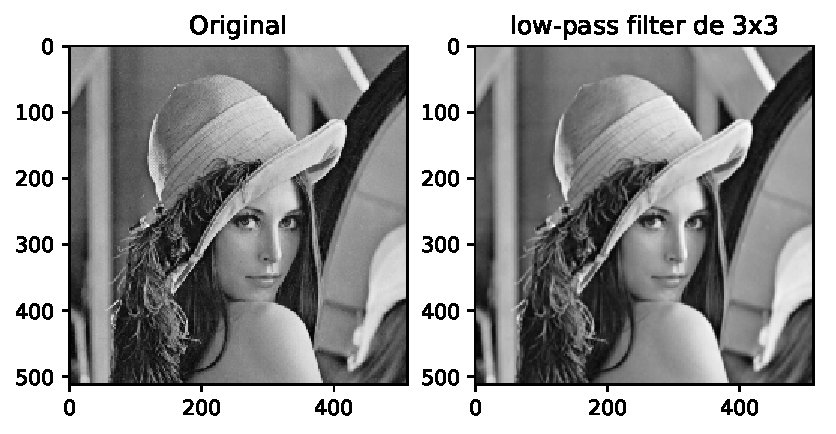
\includegraphics[height=7cm]{informe-imgs/ej1-low-3.jpg}
  \caption{\texttt{python3 practica5/ej1.py lena.png low 3}}
\end{figure}

\begin{figure}[H]
\centering
  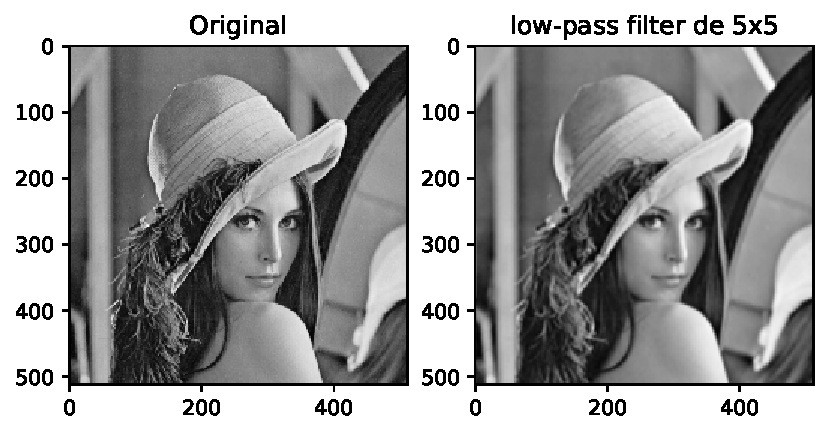
\includegraphics[height=7cm]{informe-imgs/ej1-low-5.jpg}
  \caption{\texttt{python3 practica5/ej1.py lena.png low 5}}
\end{figure}

Como puede observarse, los filtros pasa bajos son basicamente filtros que difuminan la imagen.
Esto se debe a que las máscaras toman el promedio de todos los píxeles vecinos.

\subsection{b) Máscara pasa-altos}

Usamos las siguientes máscaras (de tamaño $3 \times 3$ y $5 \times 5$ respectivamente) para el filtro pasa-bajos:

\[
\begin{bmatrix}
\frac{-1}{9} & \frac{-1}{9} & \frac{-1}{9} \\
\frac{-1}{9} & \frac{8}{9} & \frac{-1}{9} \\
\frac{-1}{9} & \frac{-1}{9} & \frac{-1}{9} \\
\end{bmatrix}
\]
\[
\begin{bmatrix}
\frac{-1}{25} & \frac{-1}{25} & \frac{-1}{25} & \frac{-1}{25} & \frac{-1}{25} \\
\frac{-1}{25} & \frac{-1}{25} & \frac{-1}{25} & \frac{-1}{25} & \frac{-1}{25} \\
\frac{-1}{25} & \frac{-1}{25} & \frac{24}{25} & \frac{-1}{25} & \frac{-1}{25} \\
\frac{-1}{25} & \frac{-1}{25} & \frac{-1}{25} & \frac{-1}{25} & \frac{-1}{25} \\
\frac{-1}{25} & \frac{-1}{25} & \frac{-1}{25} & \frac{-1}{25} & \frac{-1}{25} \\
\end{bmatrix}
\]

\begin{figure}[H]
\centering
  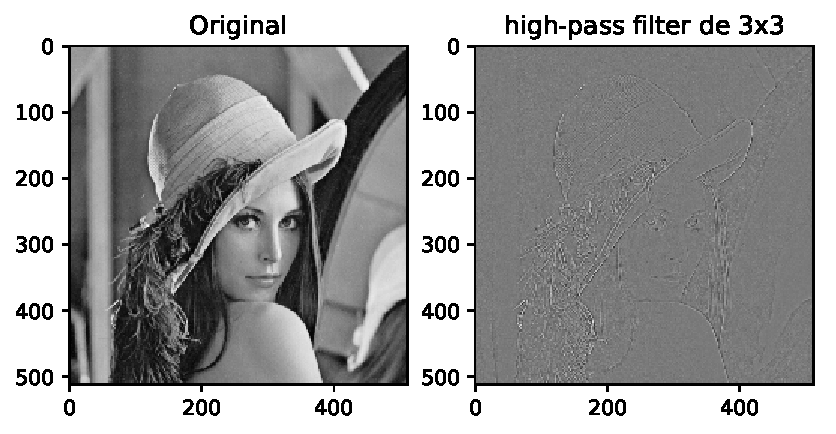
\includegraphics[height=7cm]{informe-imgs/ej1-high-3.jpg}
  \caption{\texttt{python3 practica5/ej1.py lena.png high 3}}
\end{figure}

\begin{figure}[H]
\centering
  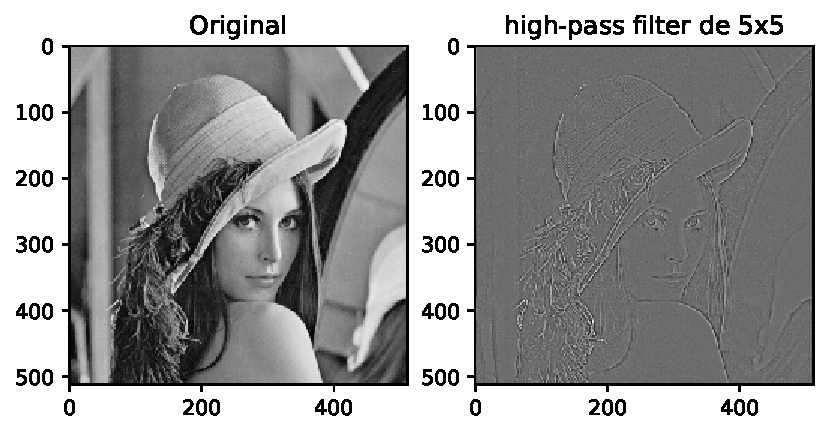
\includegraphics[height=7cm]{informe-imgs/ej1-high-5.jpg}
  \caption{\texttt{python3 practica5/ej1.py lena.png high 5}}
\end{figure}

Como puede observarse, los filtros pasa bajos son basicamente filtros que detectan bordes.
Esto se explica debido a que las frecuencias altas de la imágen
(o sea los valores asociados a los frecuencias cortas en fourier)
son los asociados a los bordes de las imágenes.

\newpage
\section{Ejercicio 2}

Implementado en el archivo \texttt{practica5/convolution.py}, junto con funciones auxiliares.

\newpage
\section{Ejercicio 3}

Aplicación de filtros variados.

Modo de uso
\begin{verbatim}
    python3 practica5/ej3.py <img1> <a|b>
\end{verbatim}

\subsection{a) Suavizado}

Para suavizar la imagen le aplicamos una convolución con la siguiente máscara:

\[
\frac{1}{273}
\begin{bmatrix}
1 & 4 & 7 & 4 & 1 \\
4 & 16 & 26 & 16 & 4 \\
7 & 26 & 41 & 26 & 7 \\
4 & 16 & 26 & 16 & 4 \\
1 & 4 & 7 & 4 & 1
\end{bmatrix}
\]

\begin{figure}[H]
\centering
  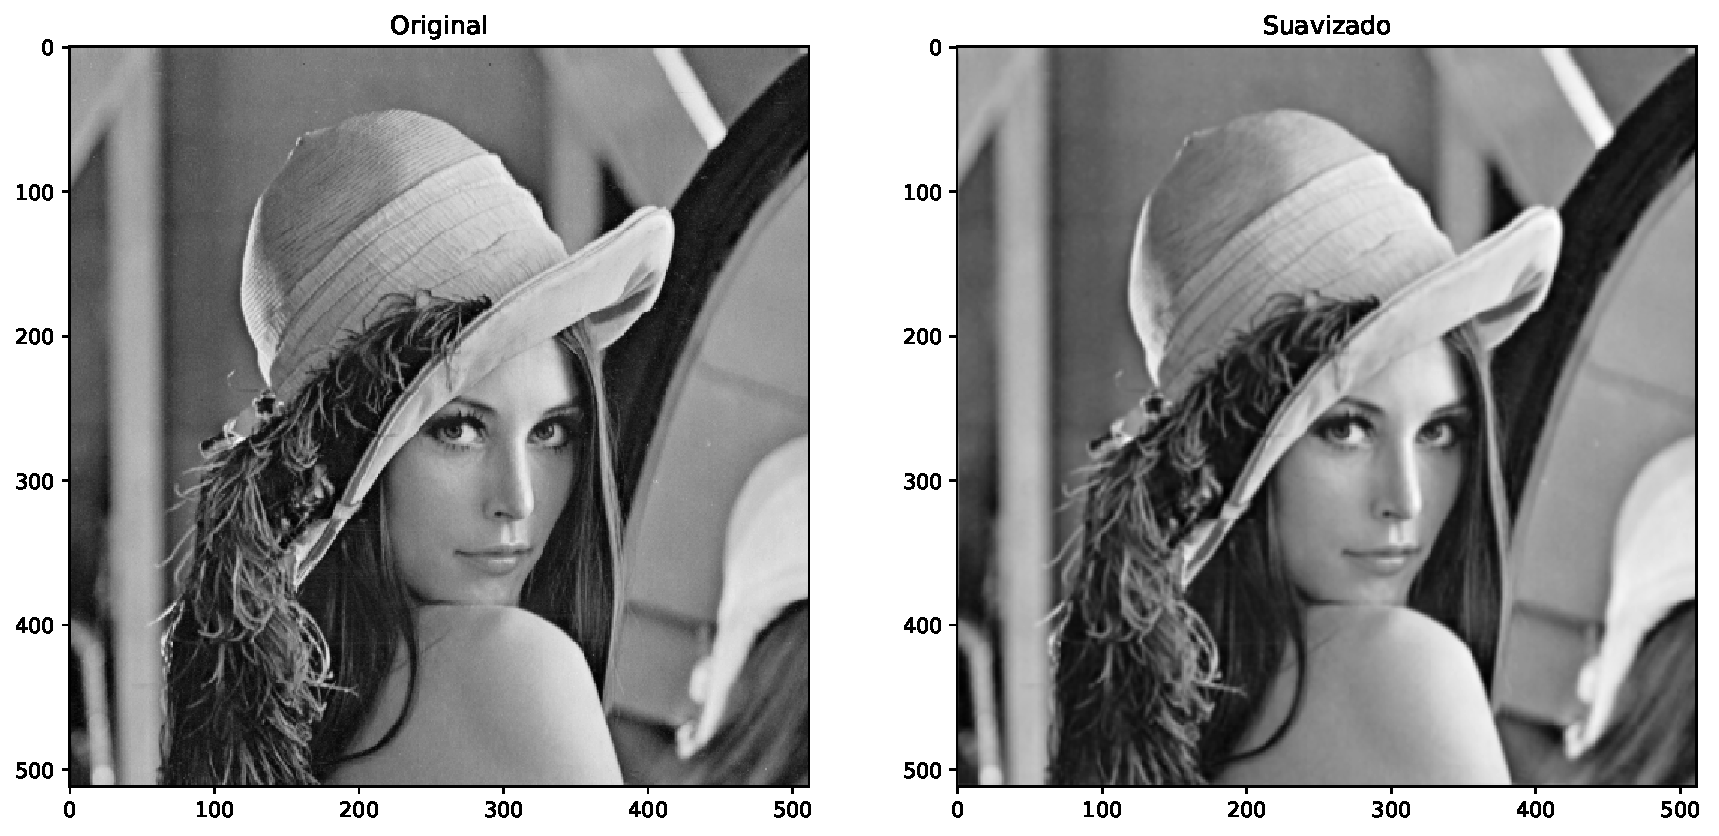
\includegraphics[height=6cm]{informe-imgs/ej3-a-lena.jpg}
  \caption{\texttt{python3 practica5/ej3.py lena.png a}}
\end{figure}


\begin{figure}[H]
\centering
  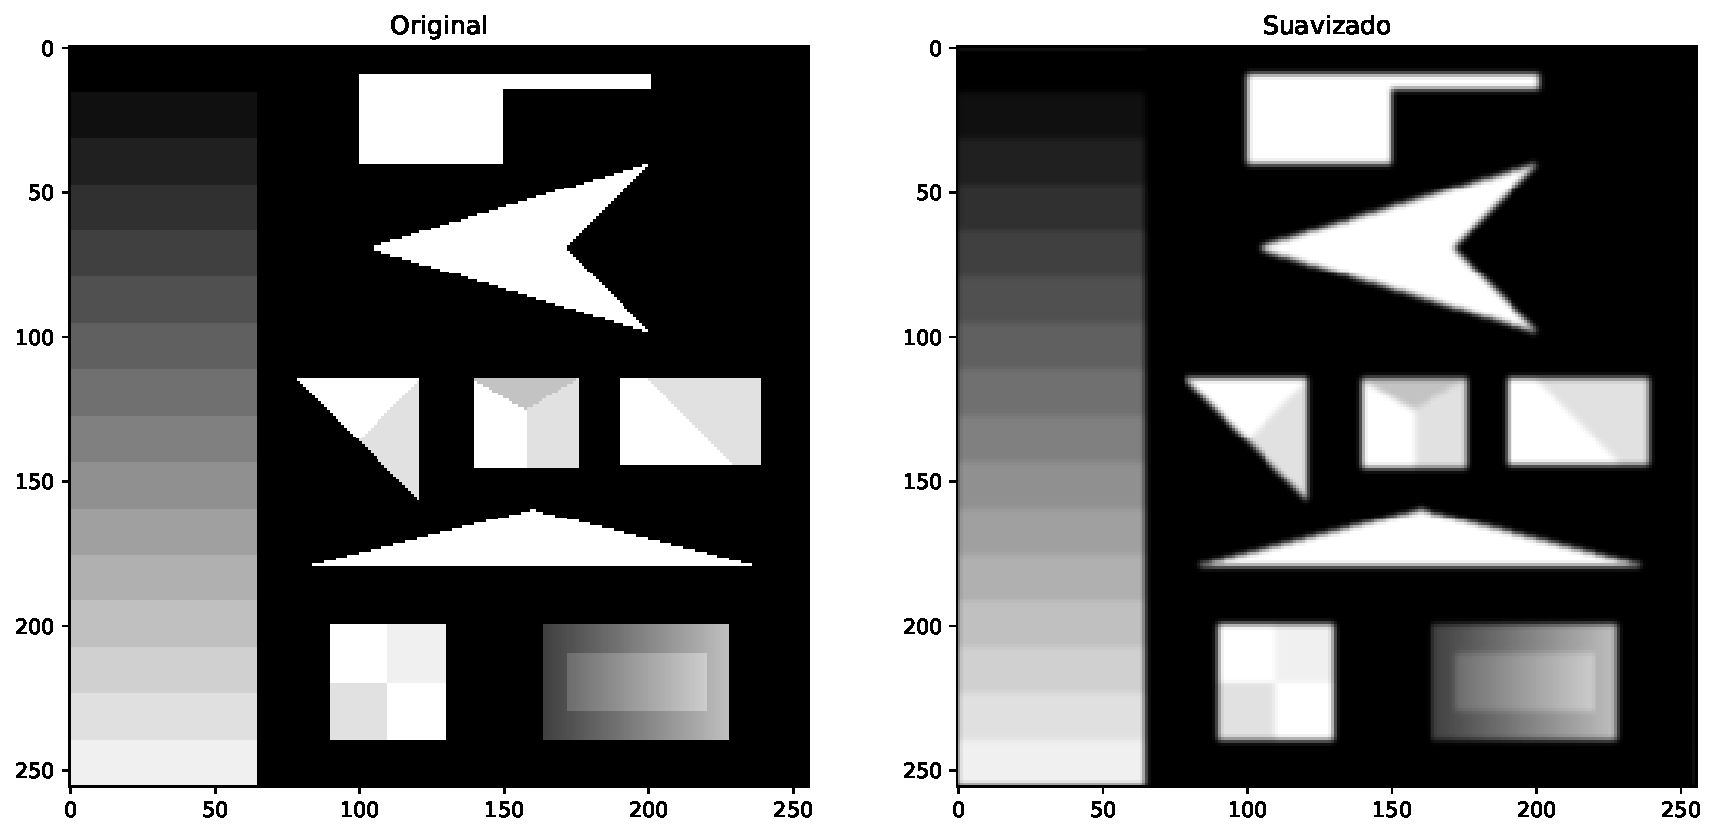
\includegraphics[height=6cm]{informe-imgs/ej3-a-test.jpg}
  \caption{\texttt{python3 practica5/ej3.py test.png a}}
\end{figure}

\subsection{b) Unsharp masking}

El filtro de unsharp masking consiste simplemente Para suavizar la imagen le aplicamos una convolución con la siguiente máscara:

\[
\frac{1}{16}
\begin{bmatrix}
-1 & -2 & -1 \\
-2 & 12 & -2 \\
-1 & -2 & -1 \\
\end{bmatrix}
\]

\noindent Y luego se la sumamos a la imágen original.

\begin{figure}[H]
\centering
  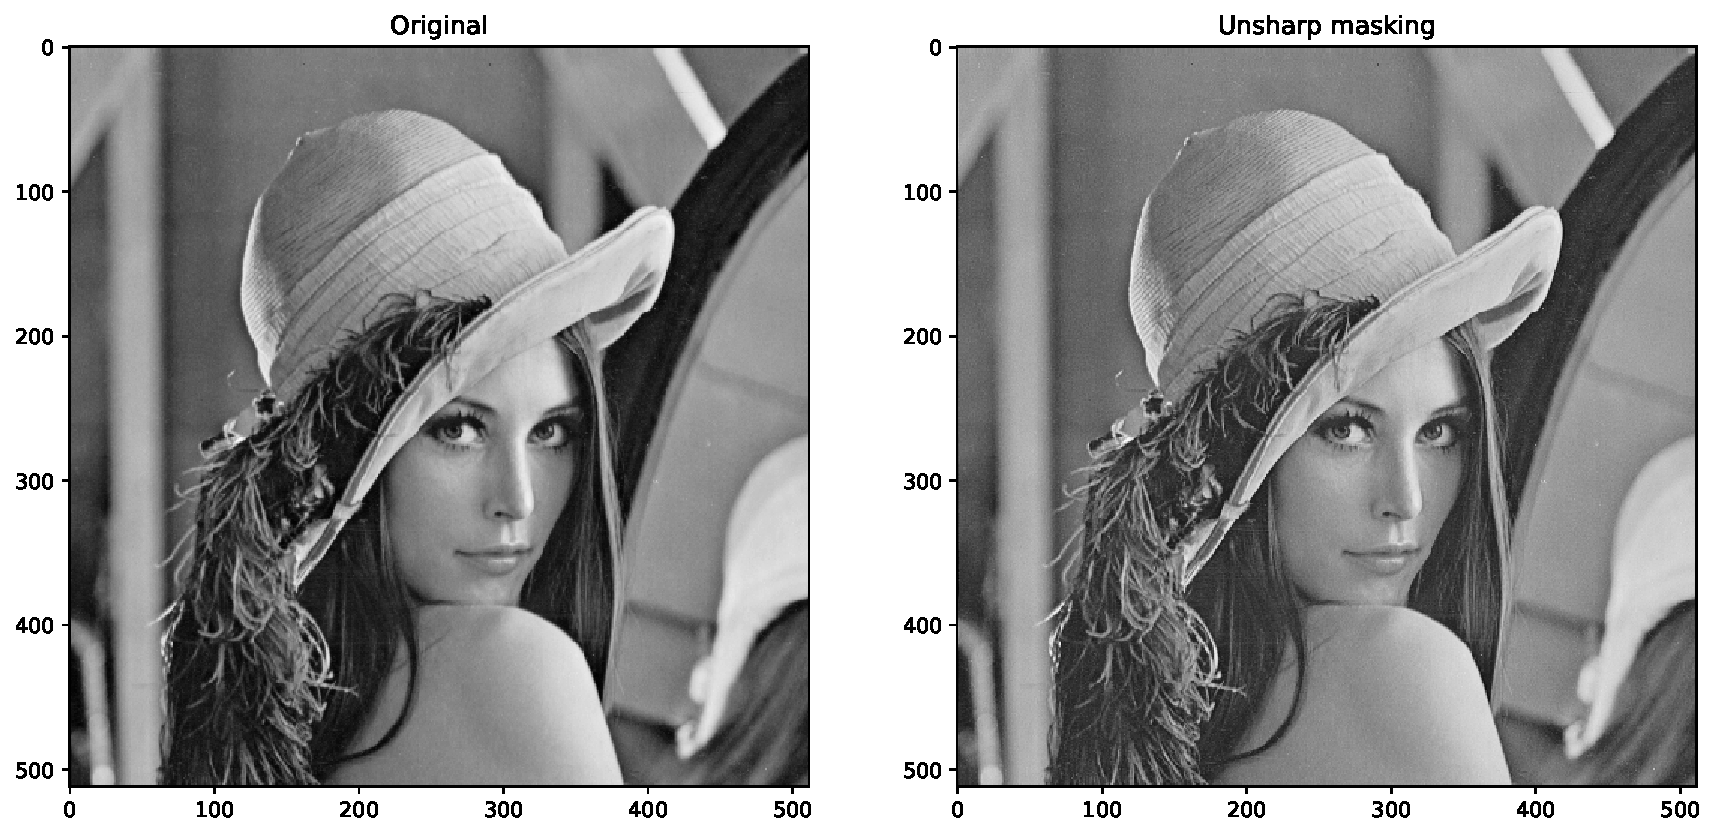
\includegraphics[height=6cm]{informe-imgs/ej3-b-lena.jpg}
  \caption{\texttt{python3 practica5/ej3.py lena.png b}}
\end{figure}


\begin{figure}[H]
\centering
  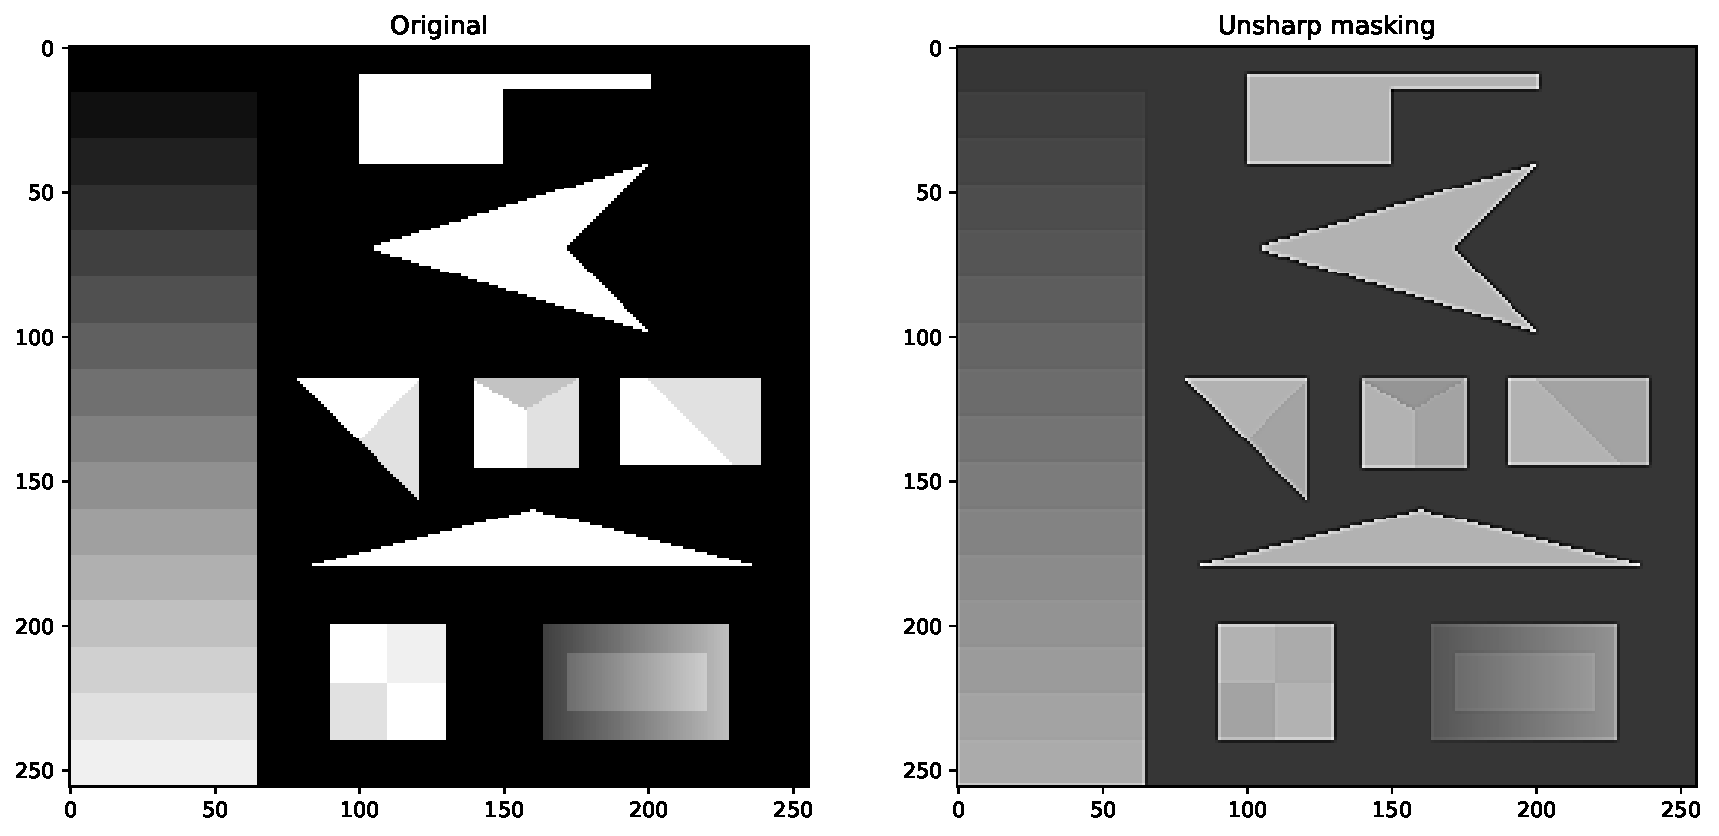
\includegraphics[height=6cm]{informe-imgs/ej3-b-test.jpg}
  \caption{\texttt{python3 practica5/ej3.py test.png b}}
\end{figure}


\newpage
\section{Ejercicio 4}

Aplicación de los filtros del ejercicio anterior a imágenes con ruidos variados.

Modo de uso
\begin{verbatim}
    python3 practica5/ej4.py <gauss|rayleigh> <param>
\end{verbatim}

Notar que el suavizado esconde el ruido bajo, mientras que el unsharp masking lo amplifica.

\subsection{a) Ruido gaussiano}

El ruido gaussiano se basa en sumarle a cada pixel el resultado de generar un número con distribución
$N(0, \sigma)$.

\begin{figure}[H]
\centering
  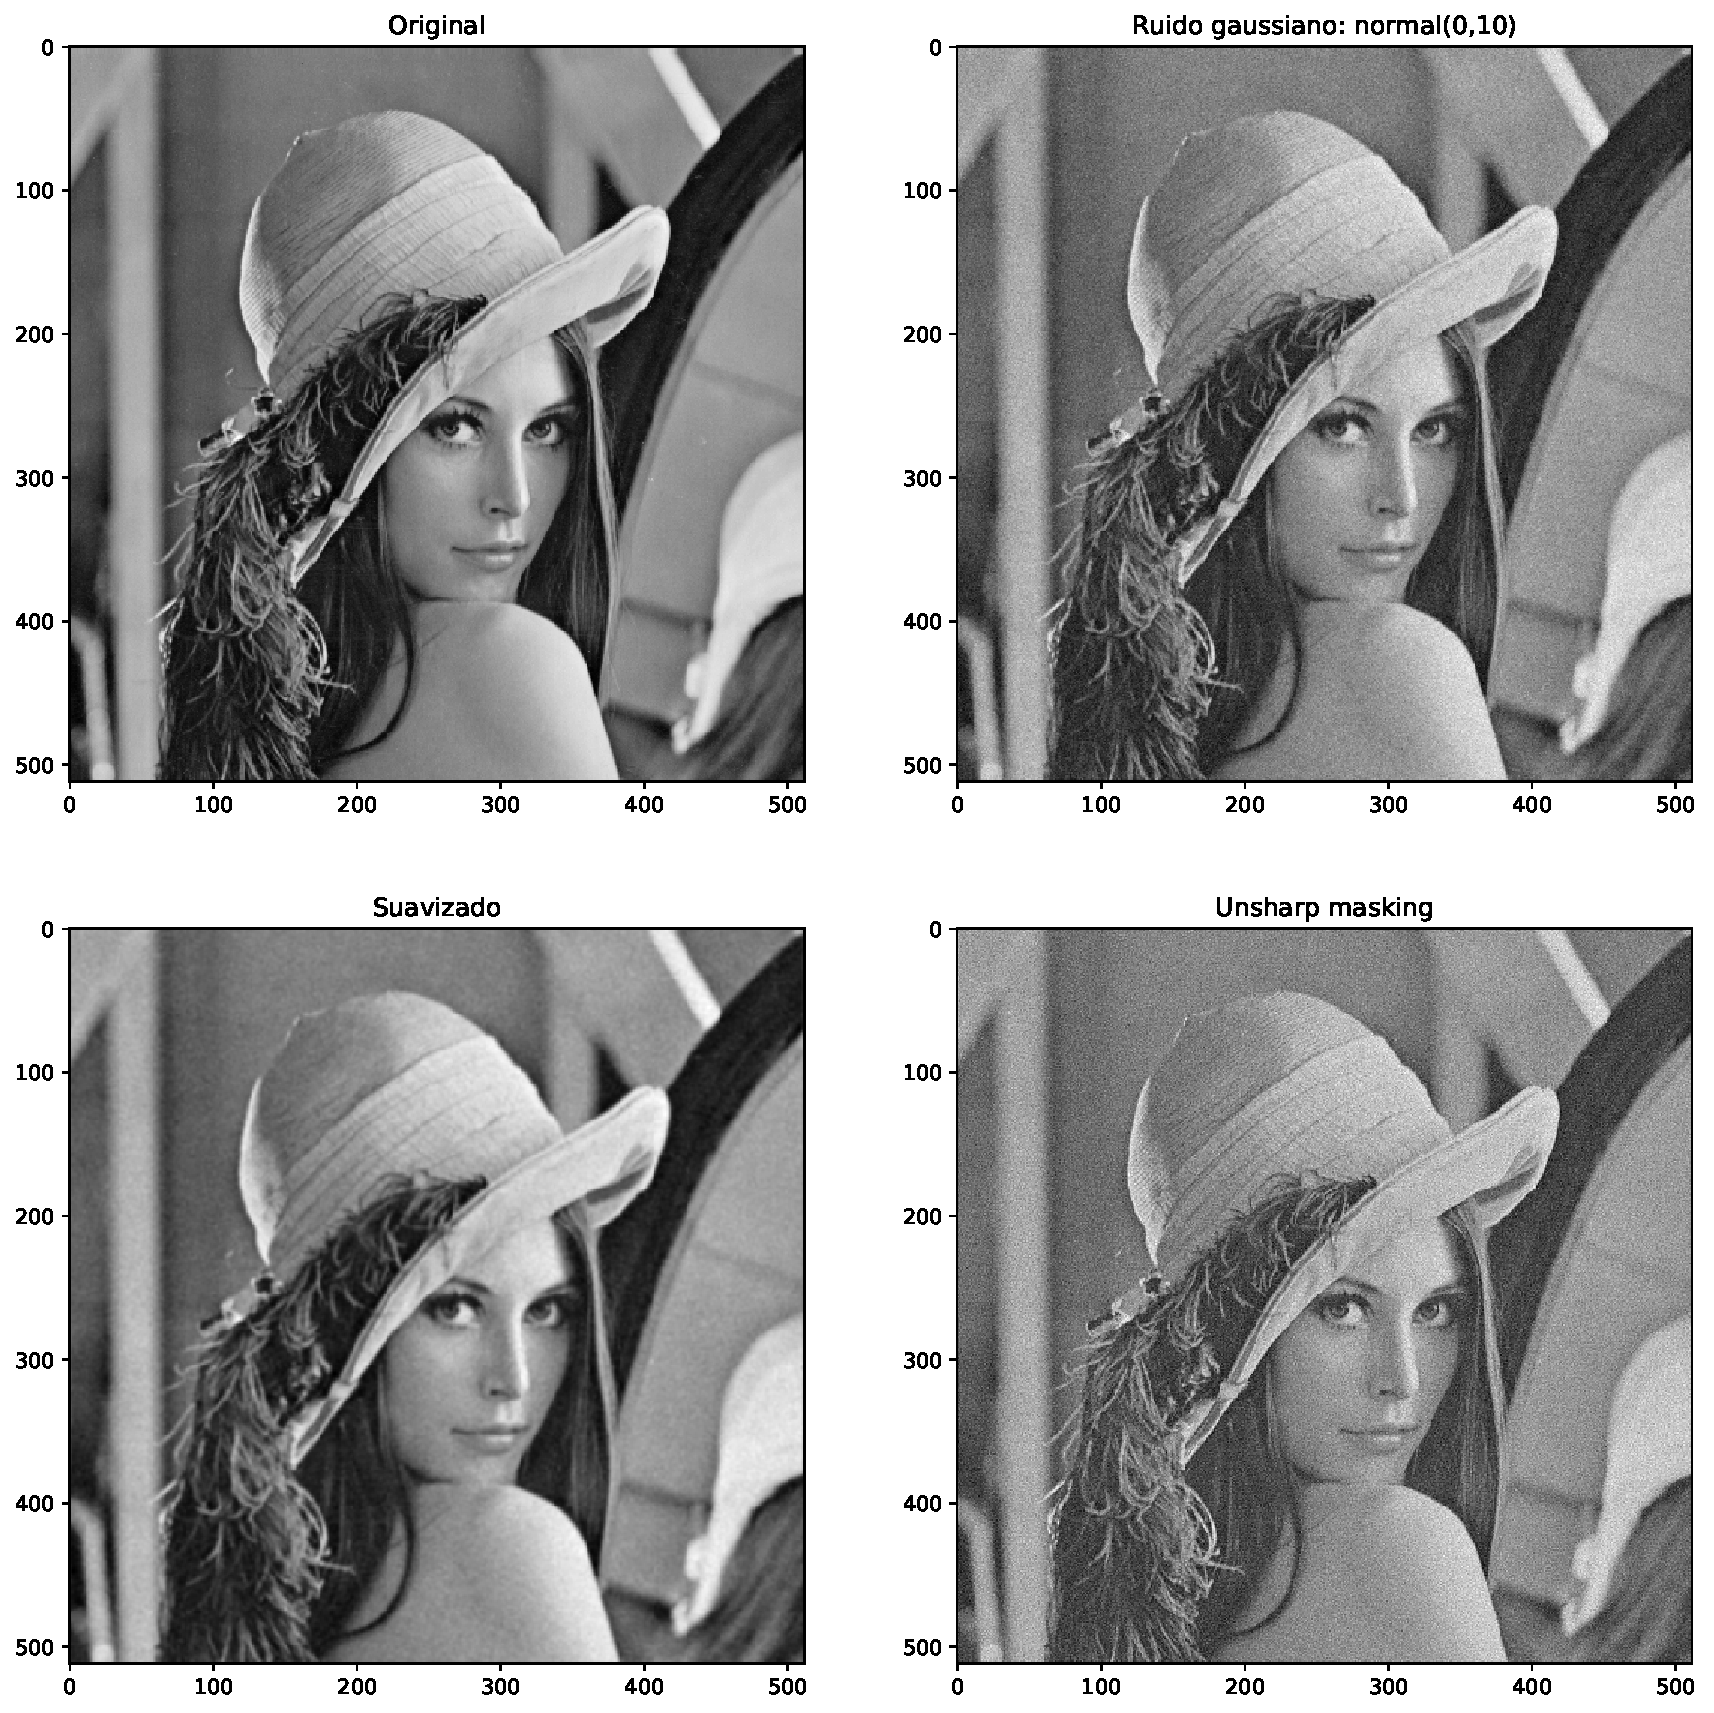
\includegraphics[height=6cm]{informe-imgs/ej4-a-lena-1.jpg}
  \caption{\texttt{python3 practica5/ej4.py lena.png gauss 10}}
\end{figure}

\begin{figure}[H]
\centering
  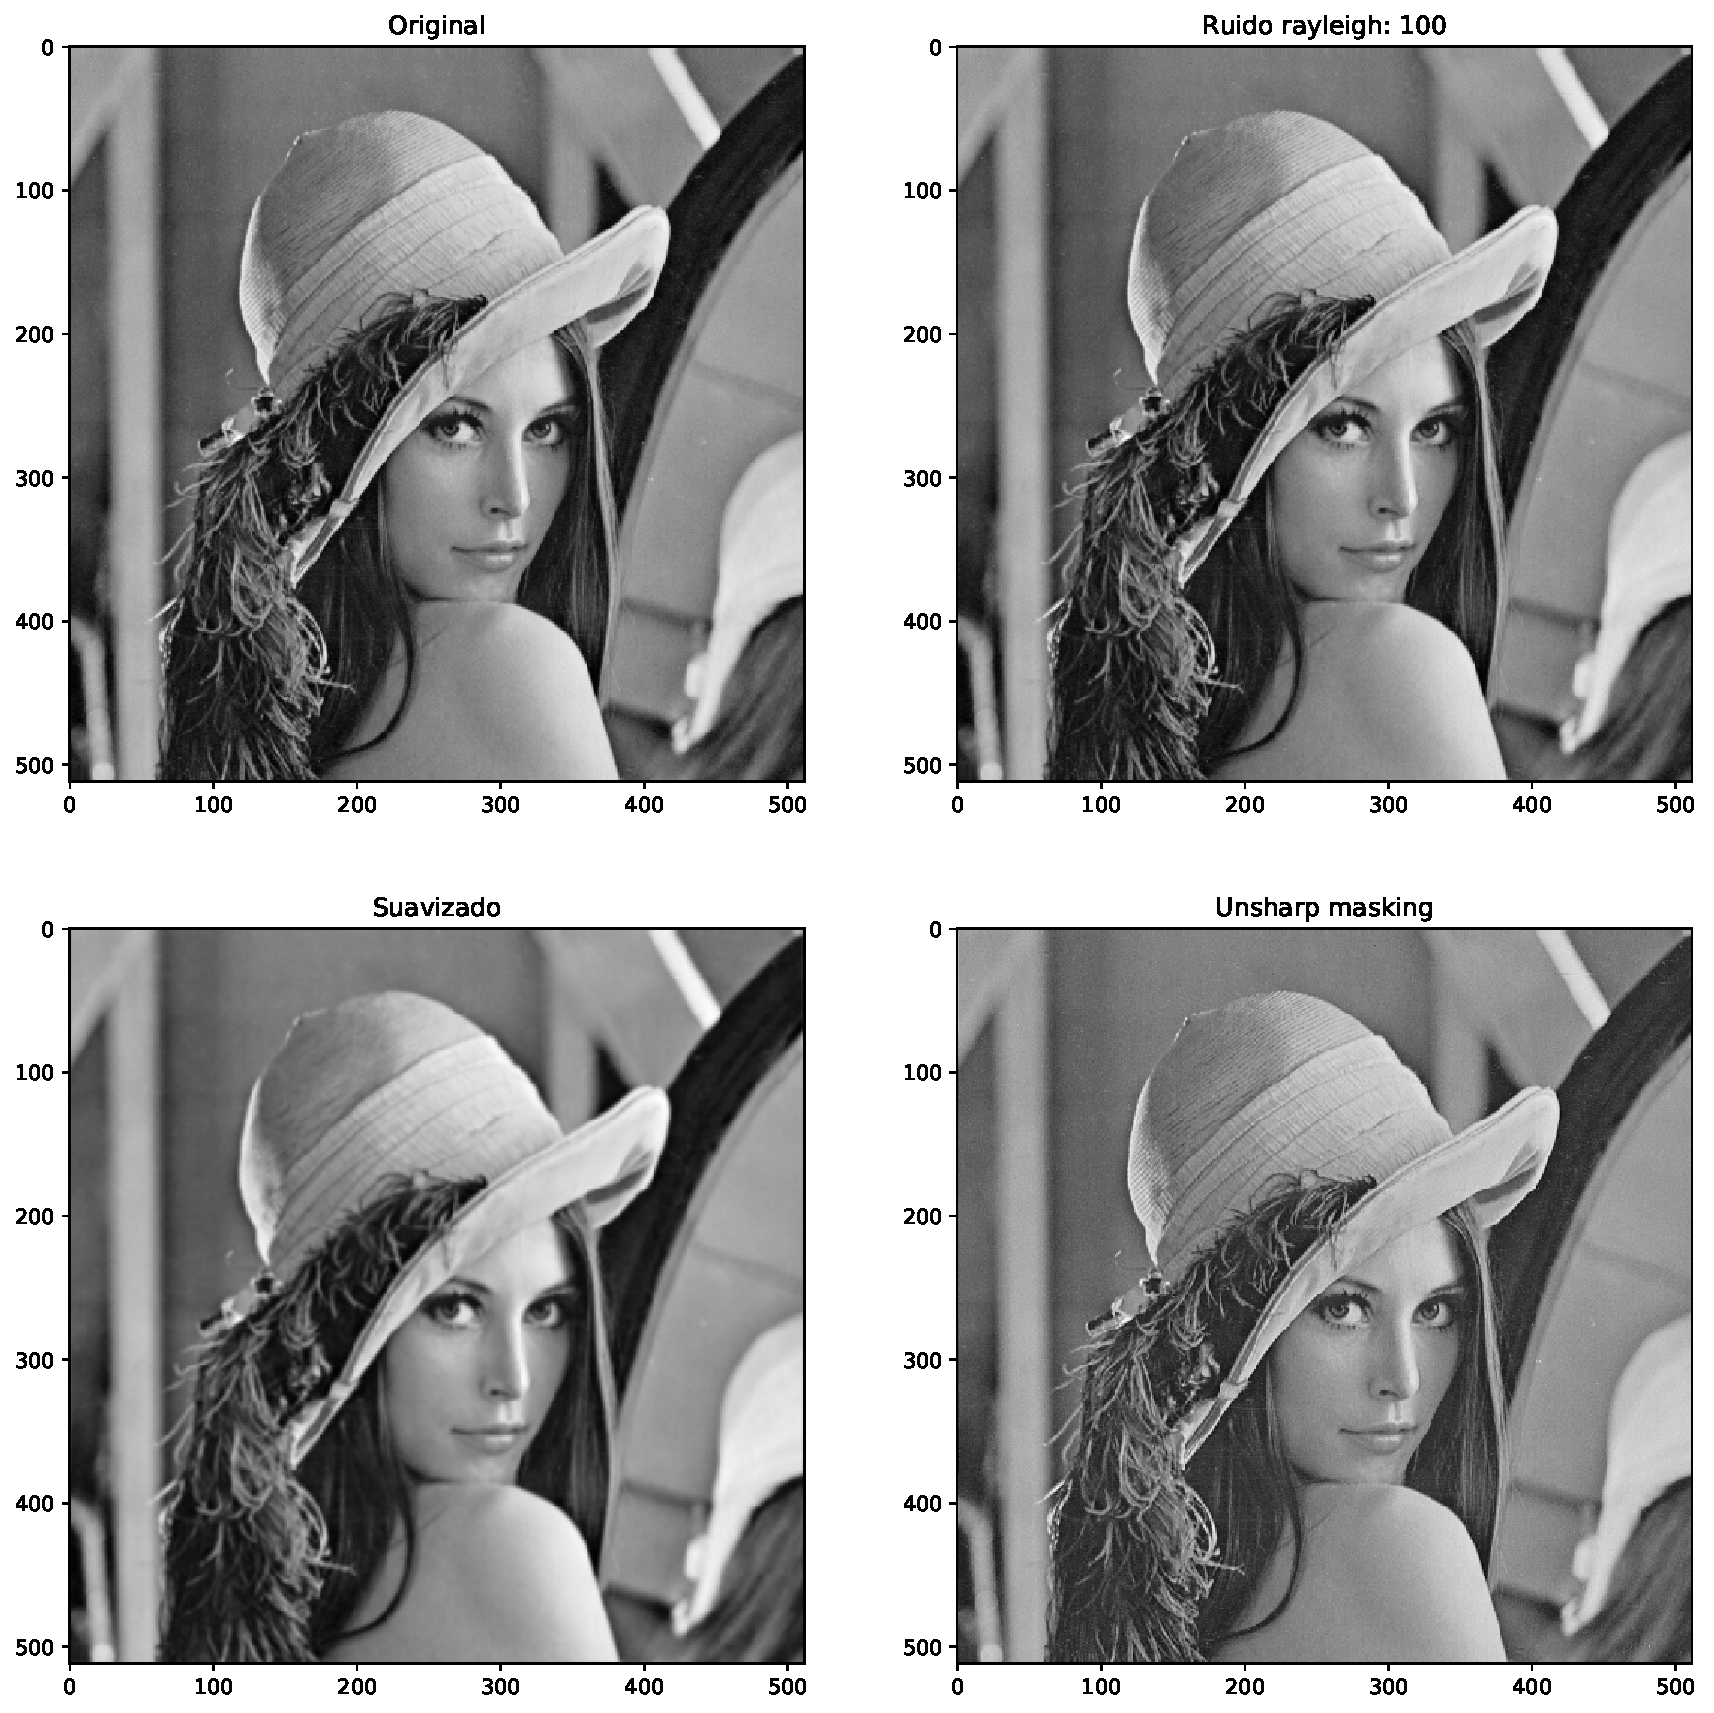
\includegraphics[height=6cm]{informe-imgs/ej4-a-lena-2.jpg}
  \caption{\texttt{python3 practica5/ej4.py lena.png rayleigh 100}}
\end{figure}

\subsection{b) Ruido Rayleigh}

El ruido gaussiano se basa en sumarle a cada pixel el resultado de generar un número con distribución Rayleigh.

\begin{figure}[H]
\centering
  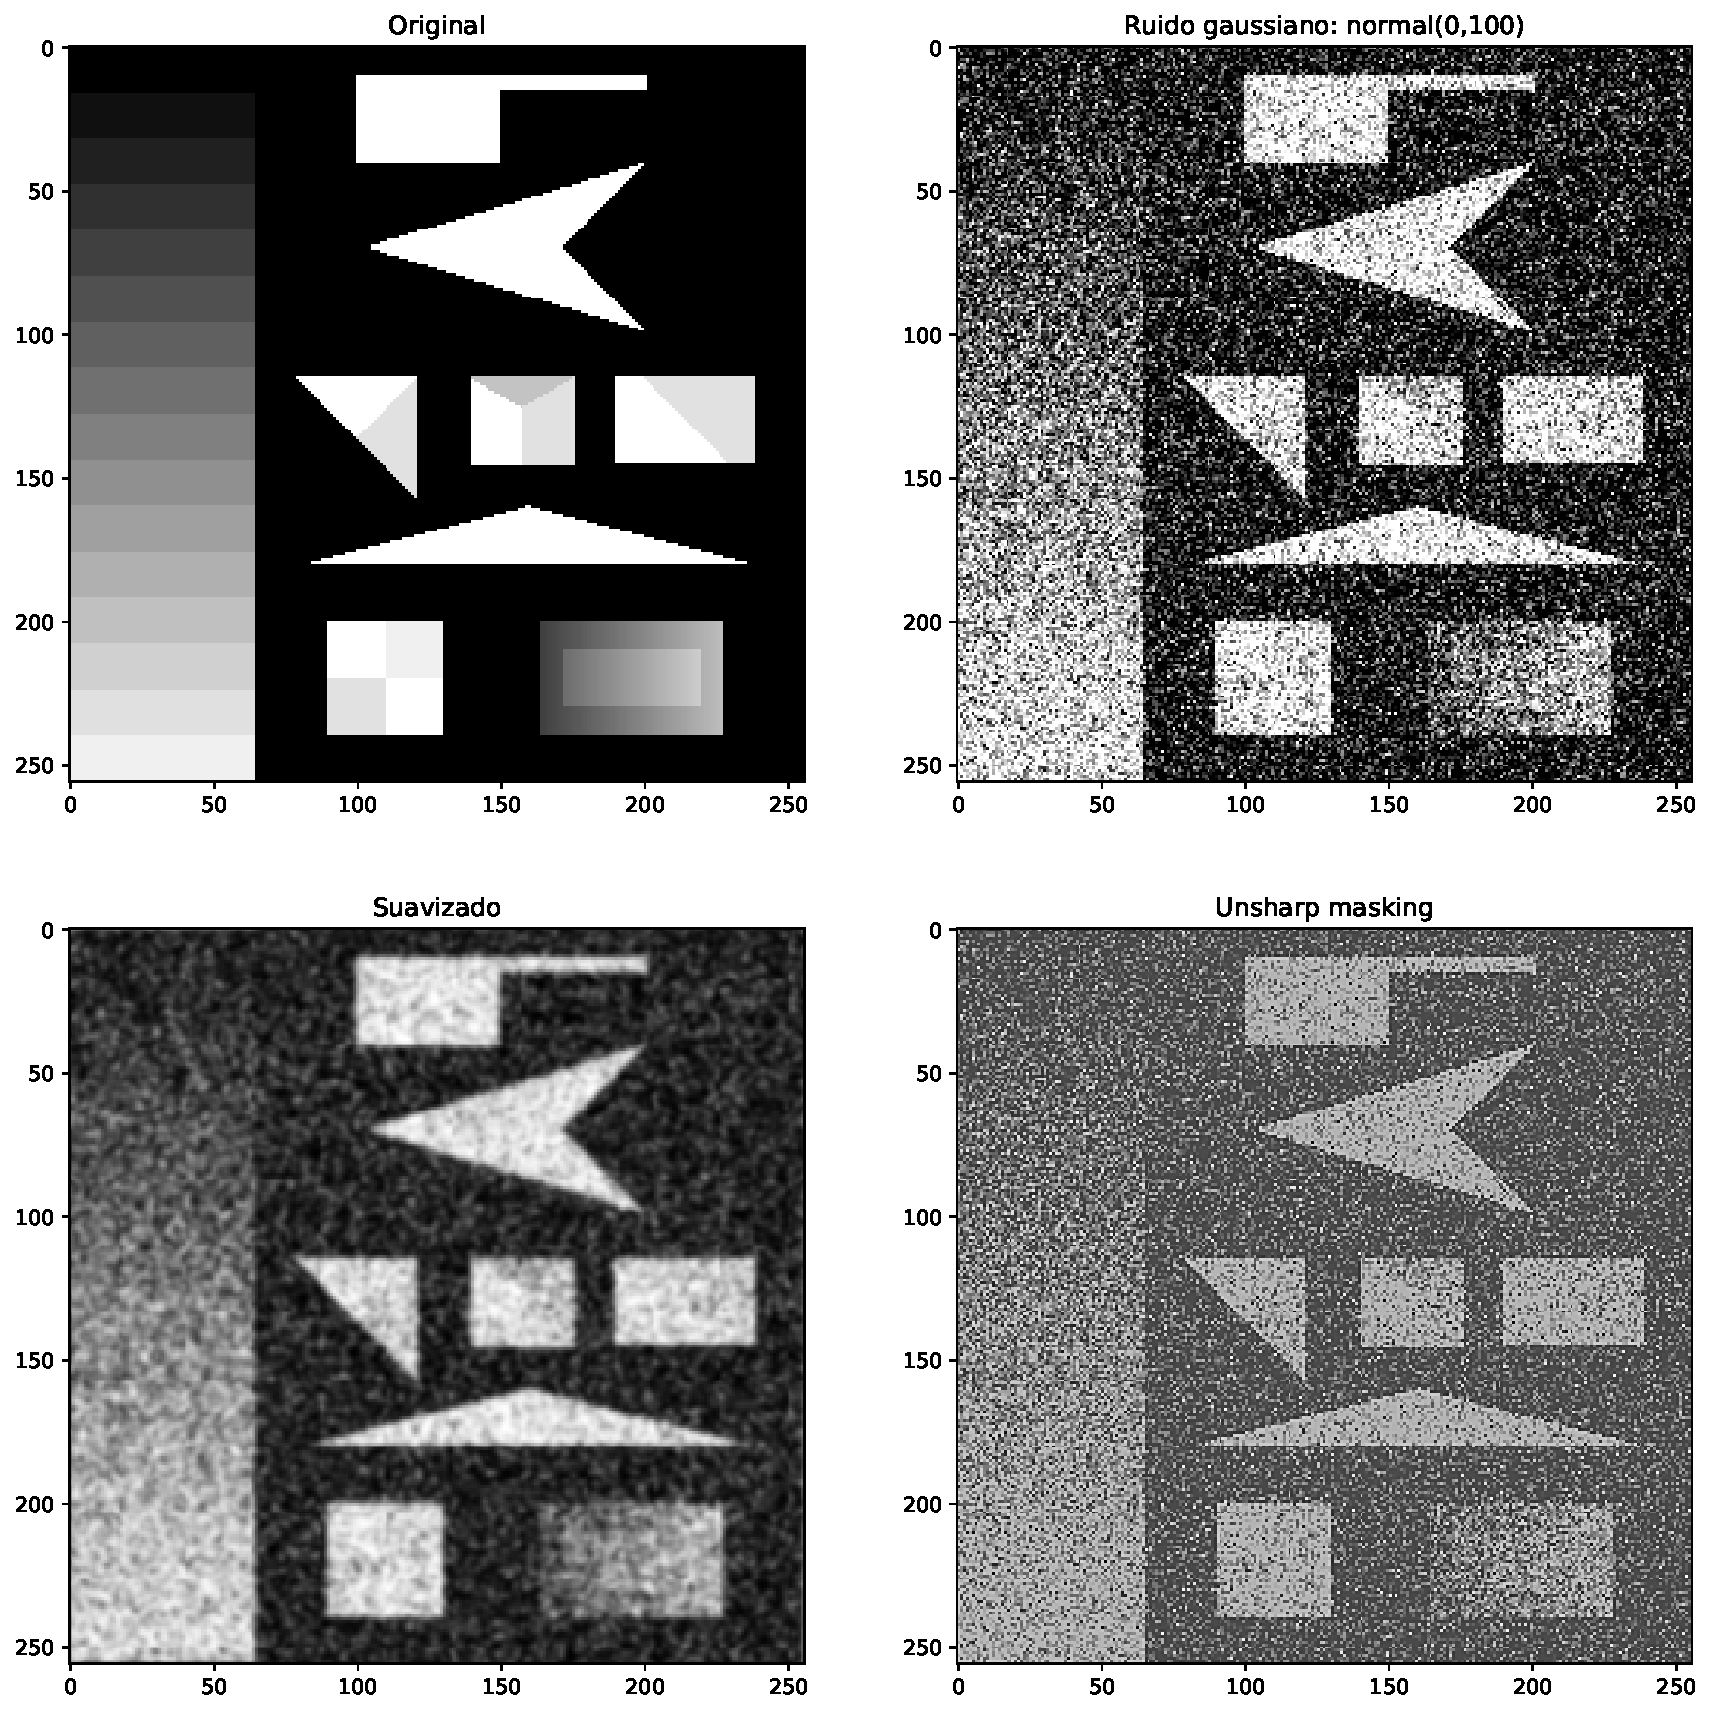
\includegraphics[height=6cm]{informe-imgs/ej4-b-test-1.jpg}
  \caption{\texttt{python3 practica5/ej4.py lena.png gauss 100}}
\end{figure}

\begin{figure}[H]
\centering
  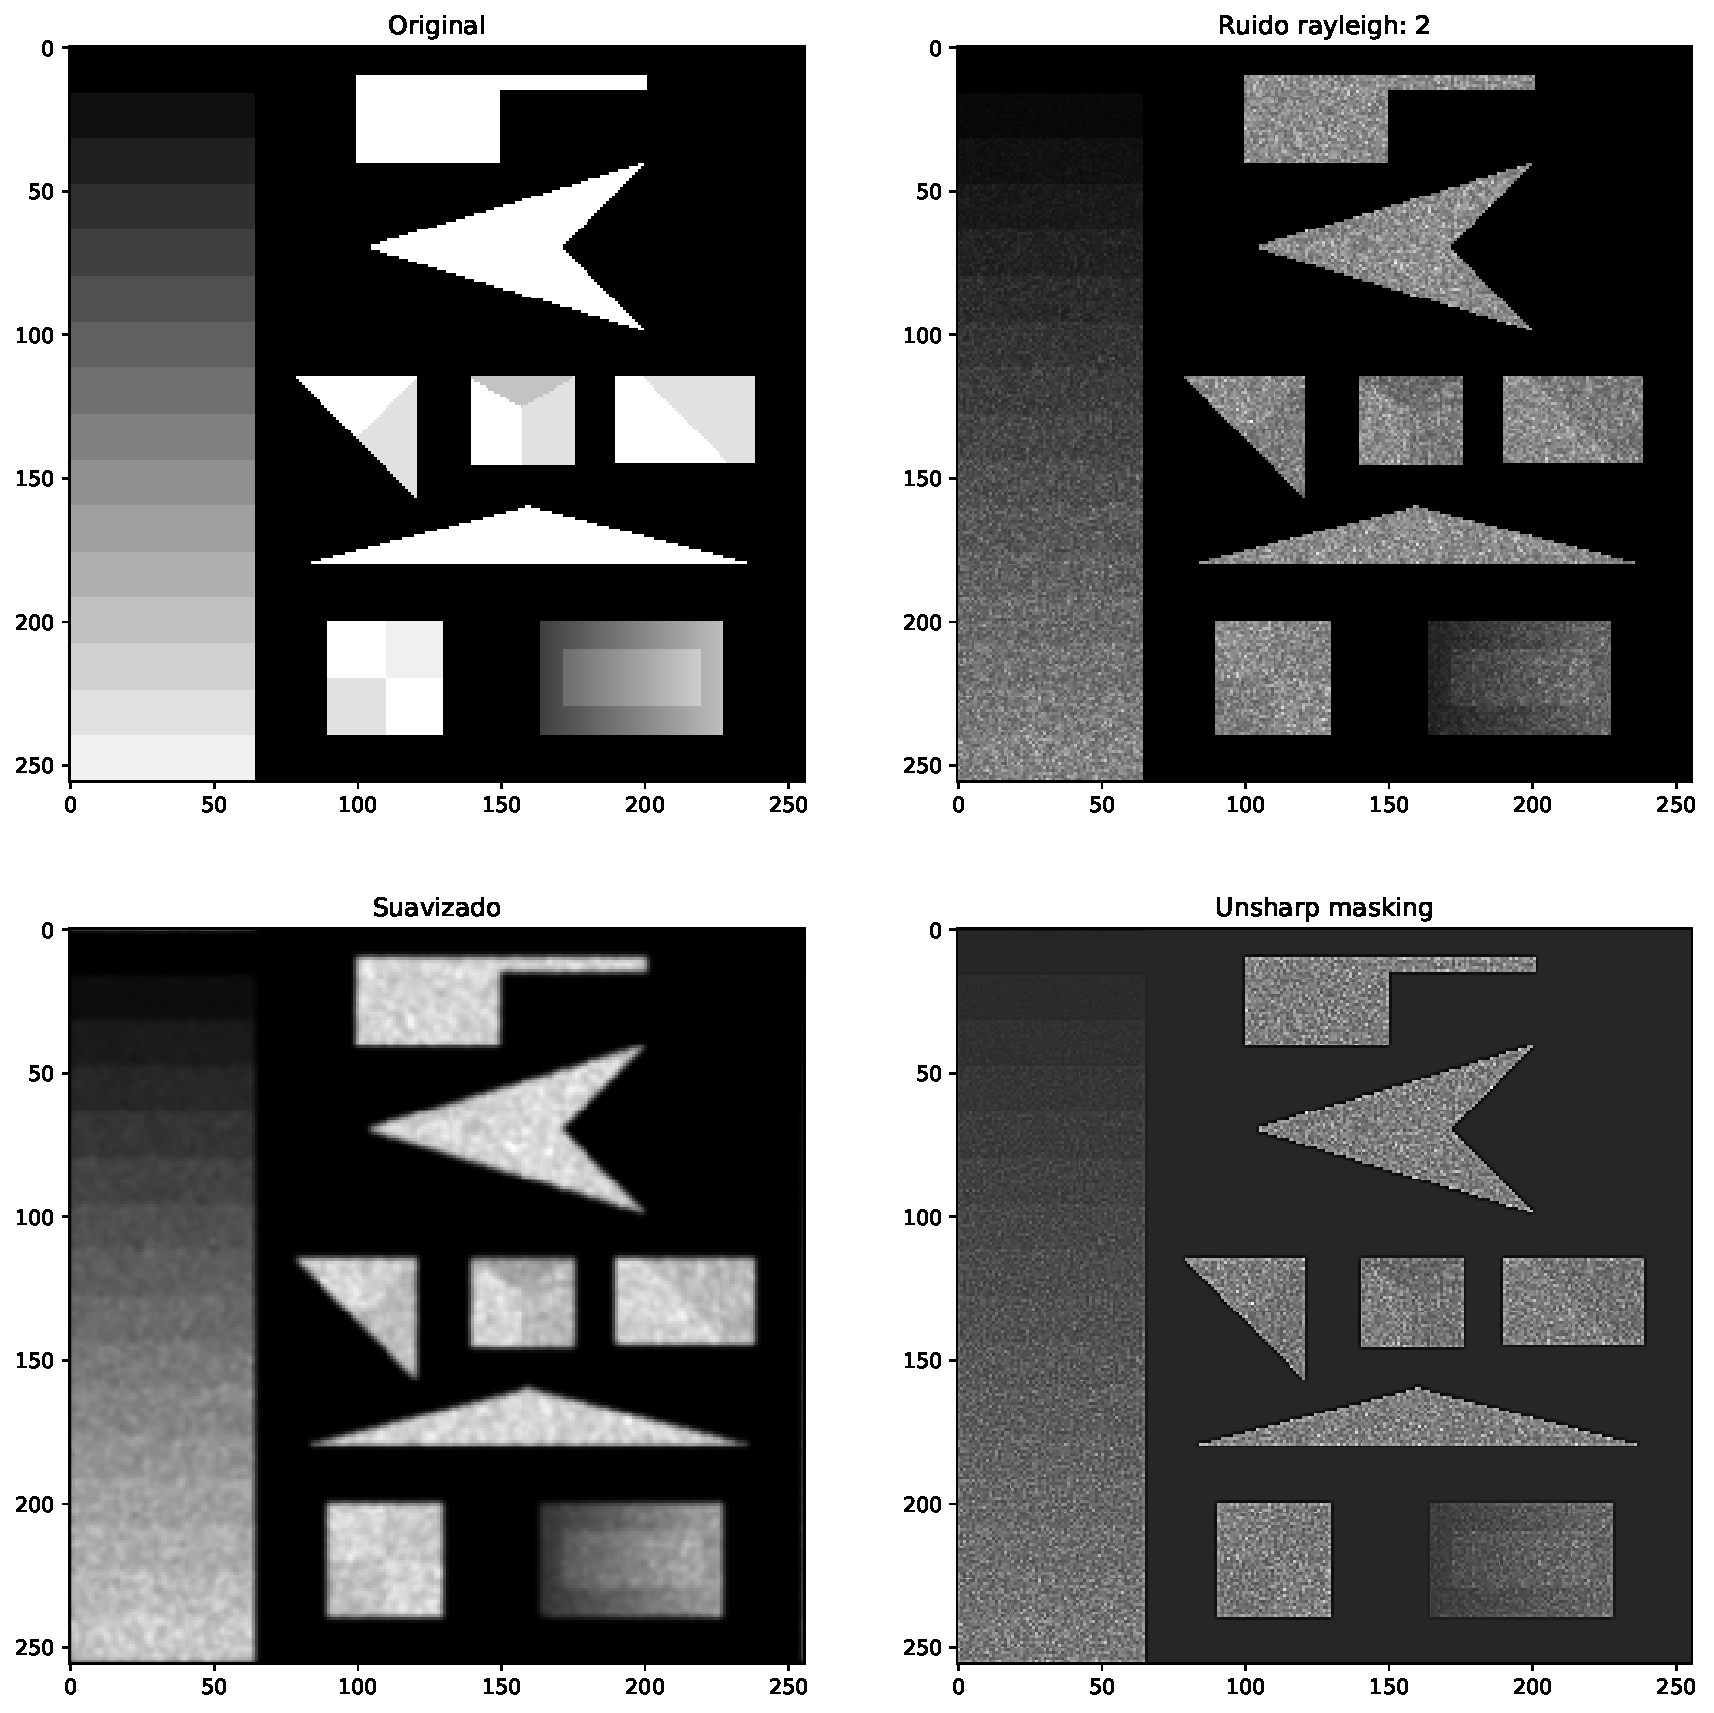
\includegraphics[height=6cm]{informe-imgs/ej4-b-test-2.jpg}
  \caption{\texttt{python3 practica5/ej4.py lena.png rayleigh 2}}
\end{figure}

\newpage
\section{Ejercicios 5 y 6}

Filtro de la mediana, y su aplicación a imágenes con ruido.

Modo de uso
\begin{verbatim}
    python3 practica5/ej5.py <img> <param_gauss> <param_salt_pepper>
\end{verbatim}

Notar que el filtro de la mediana permite eliminar el ruido salt \& pepper casi completamente cuando
tiene probabilidad baja.

Tambien ayuda a mejorar las imágenes con ruido gaussiano, aunque no las restaura del todo.


\textbf{Ruido bajo}

\begin{figure}[H]
\centering
  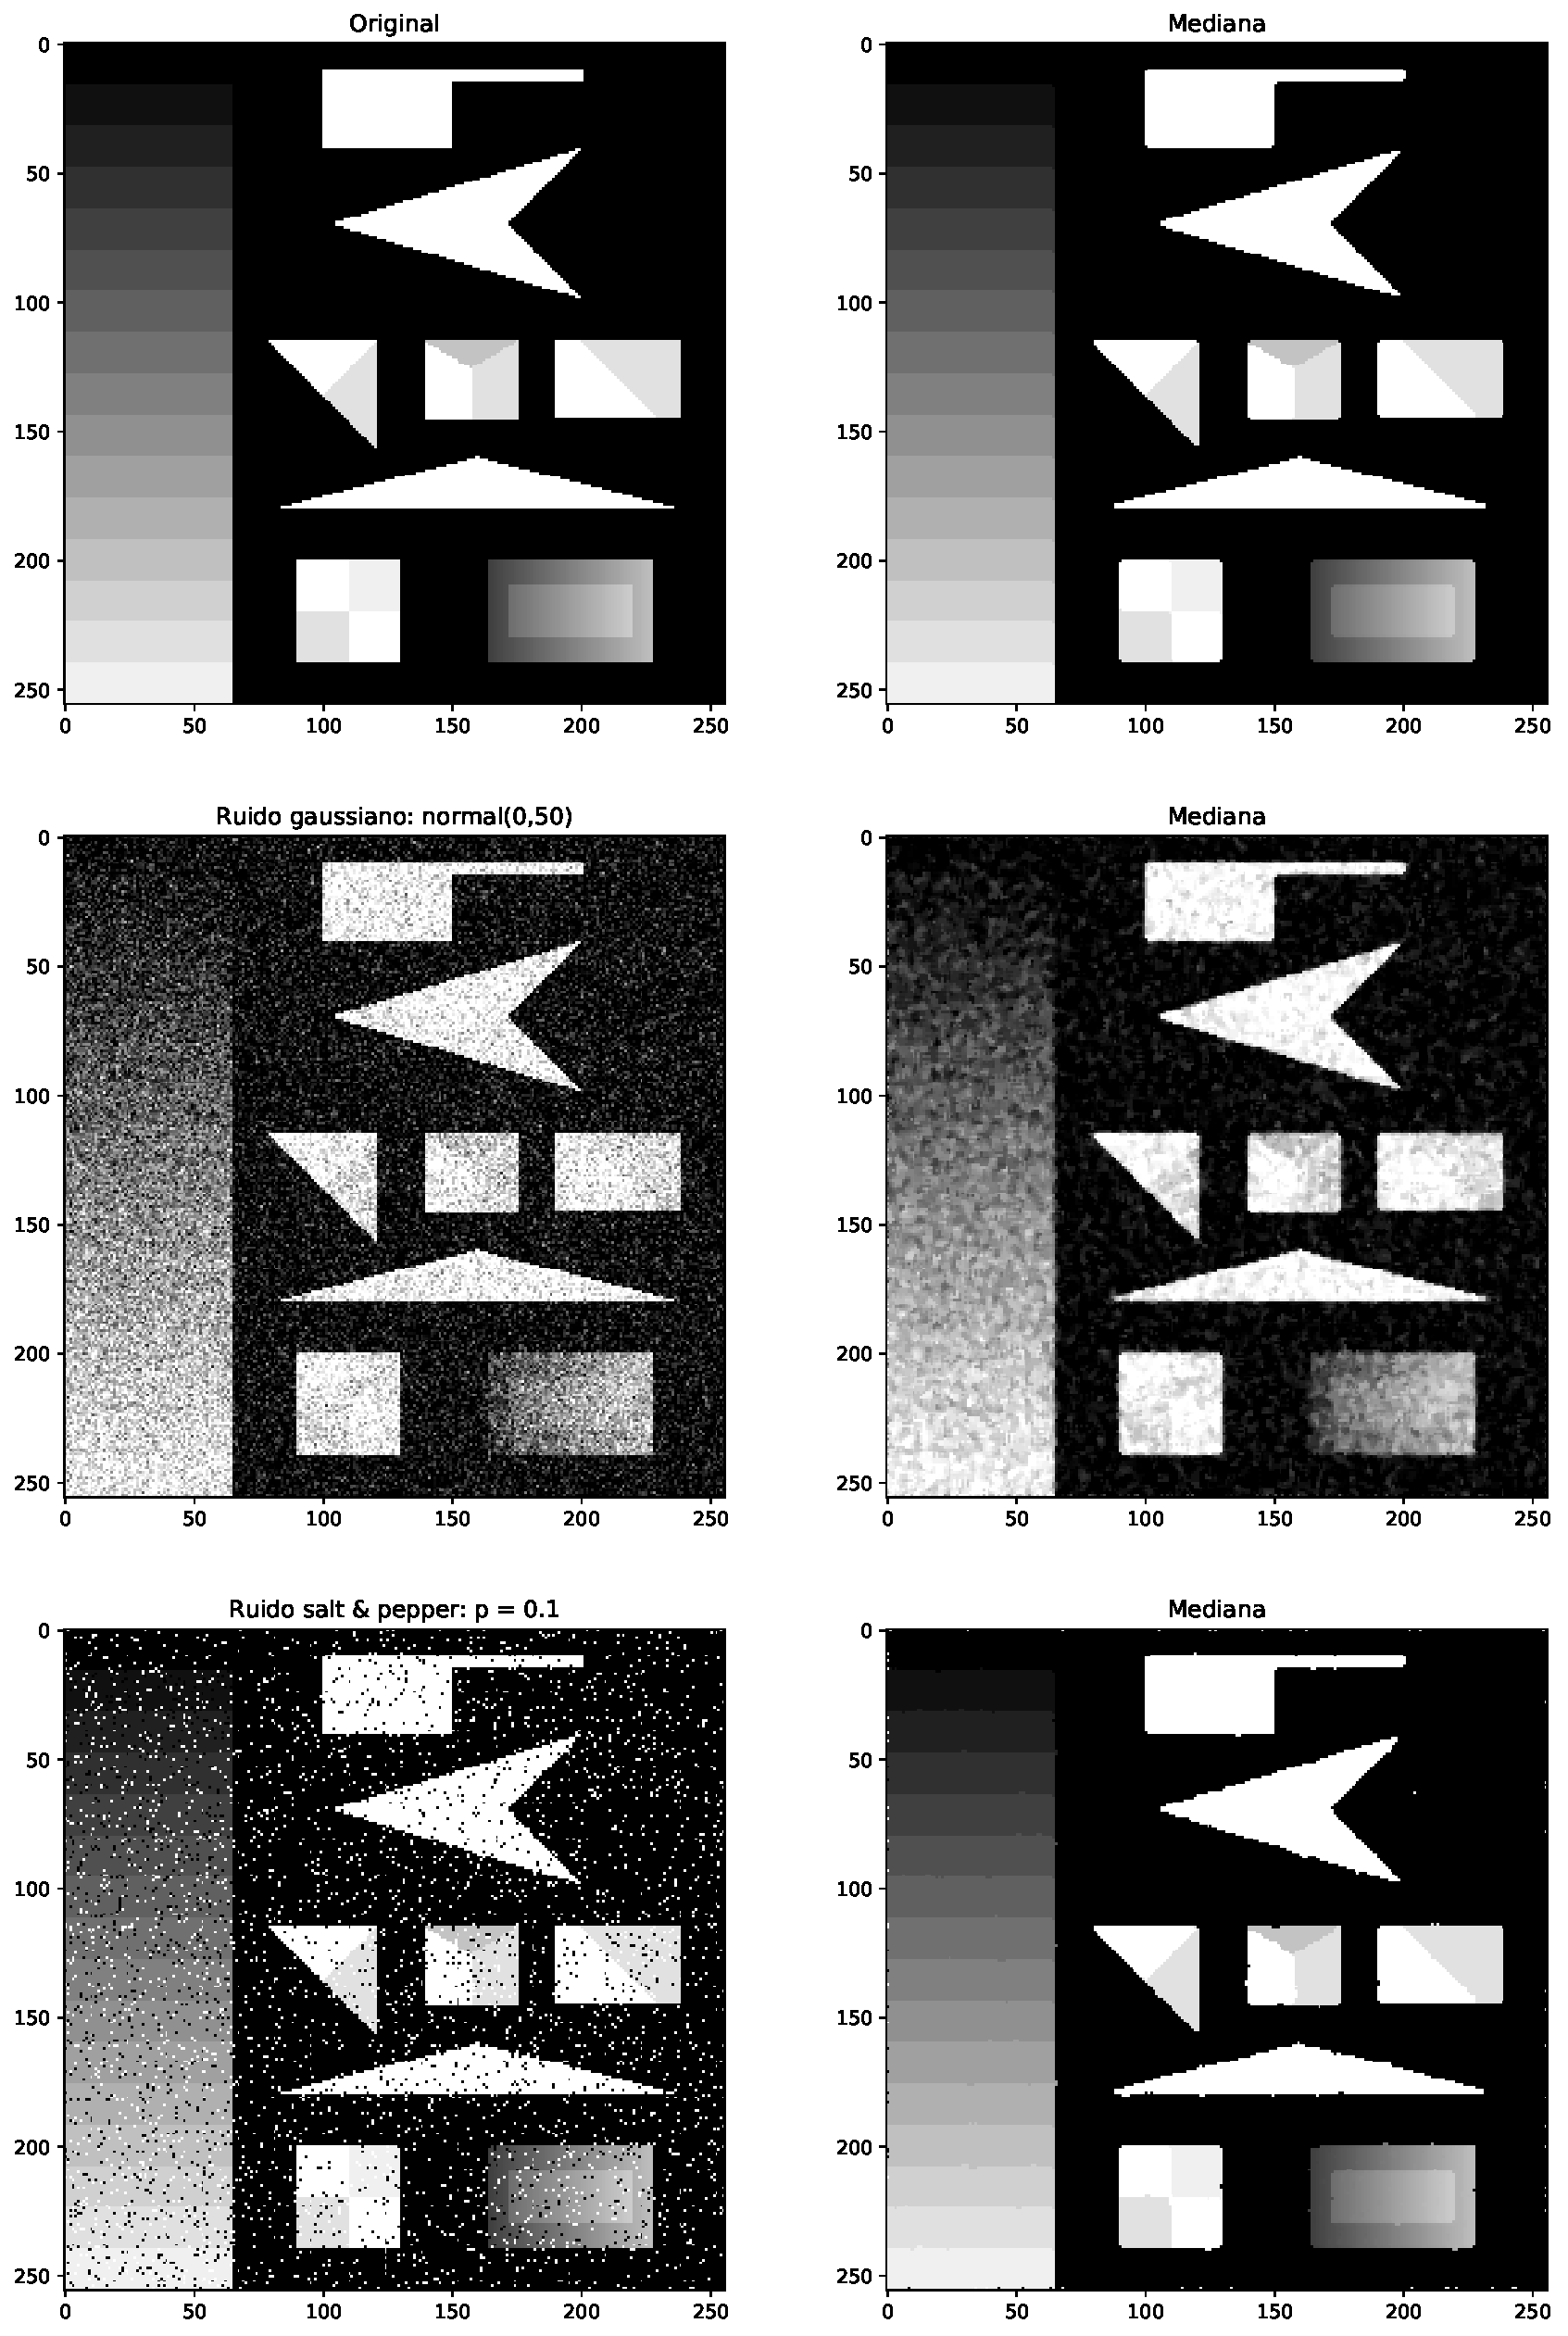
\includegraphics[height=10cm]{informe-imgs/ej6-1.jpg}
  \caption{\texttt{python3 practica5/ej5.py test.png 50 0.1}}
\end{figure}

\begin{figure}[H]
\centering
  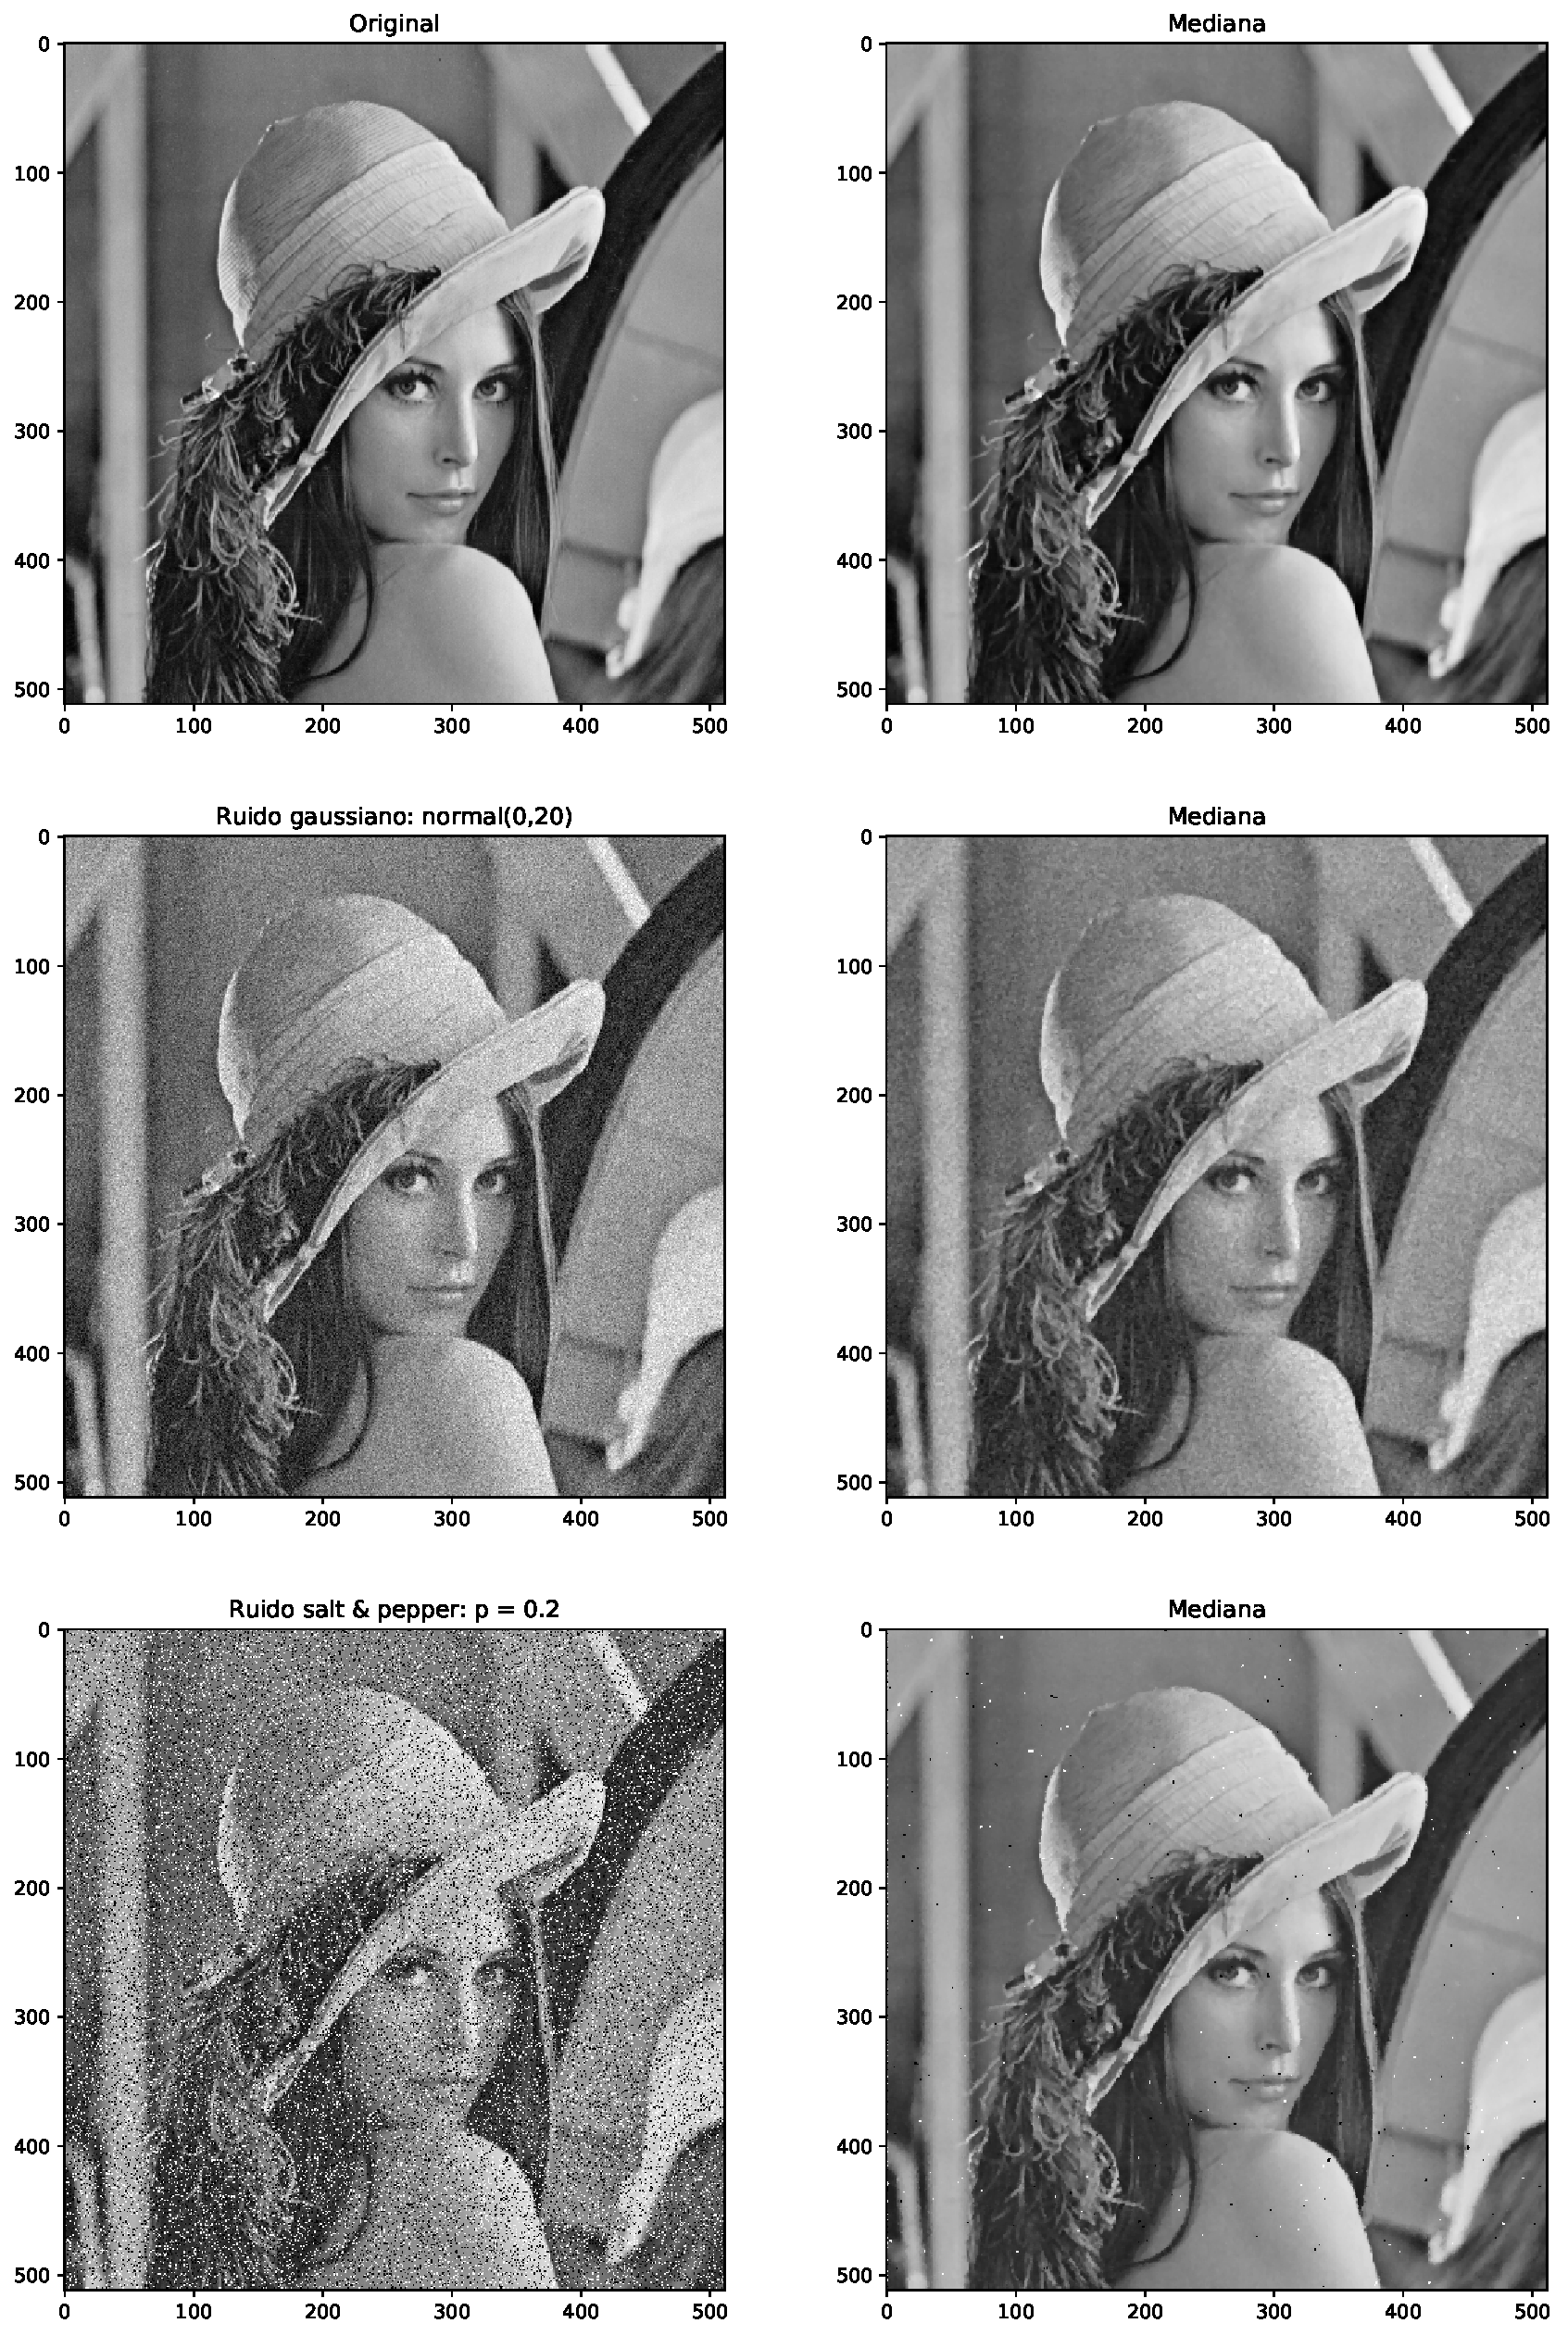
\includegraphics[height=10cm]{informe-imgs/ej6-2.jpg}
  \caption{\texttt{python3 practica5/ej5.py lena.png 20 0.2}}
\end{figure}

\textbf{Ruido alto}

\begin{figure}[H]
\centering
  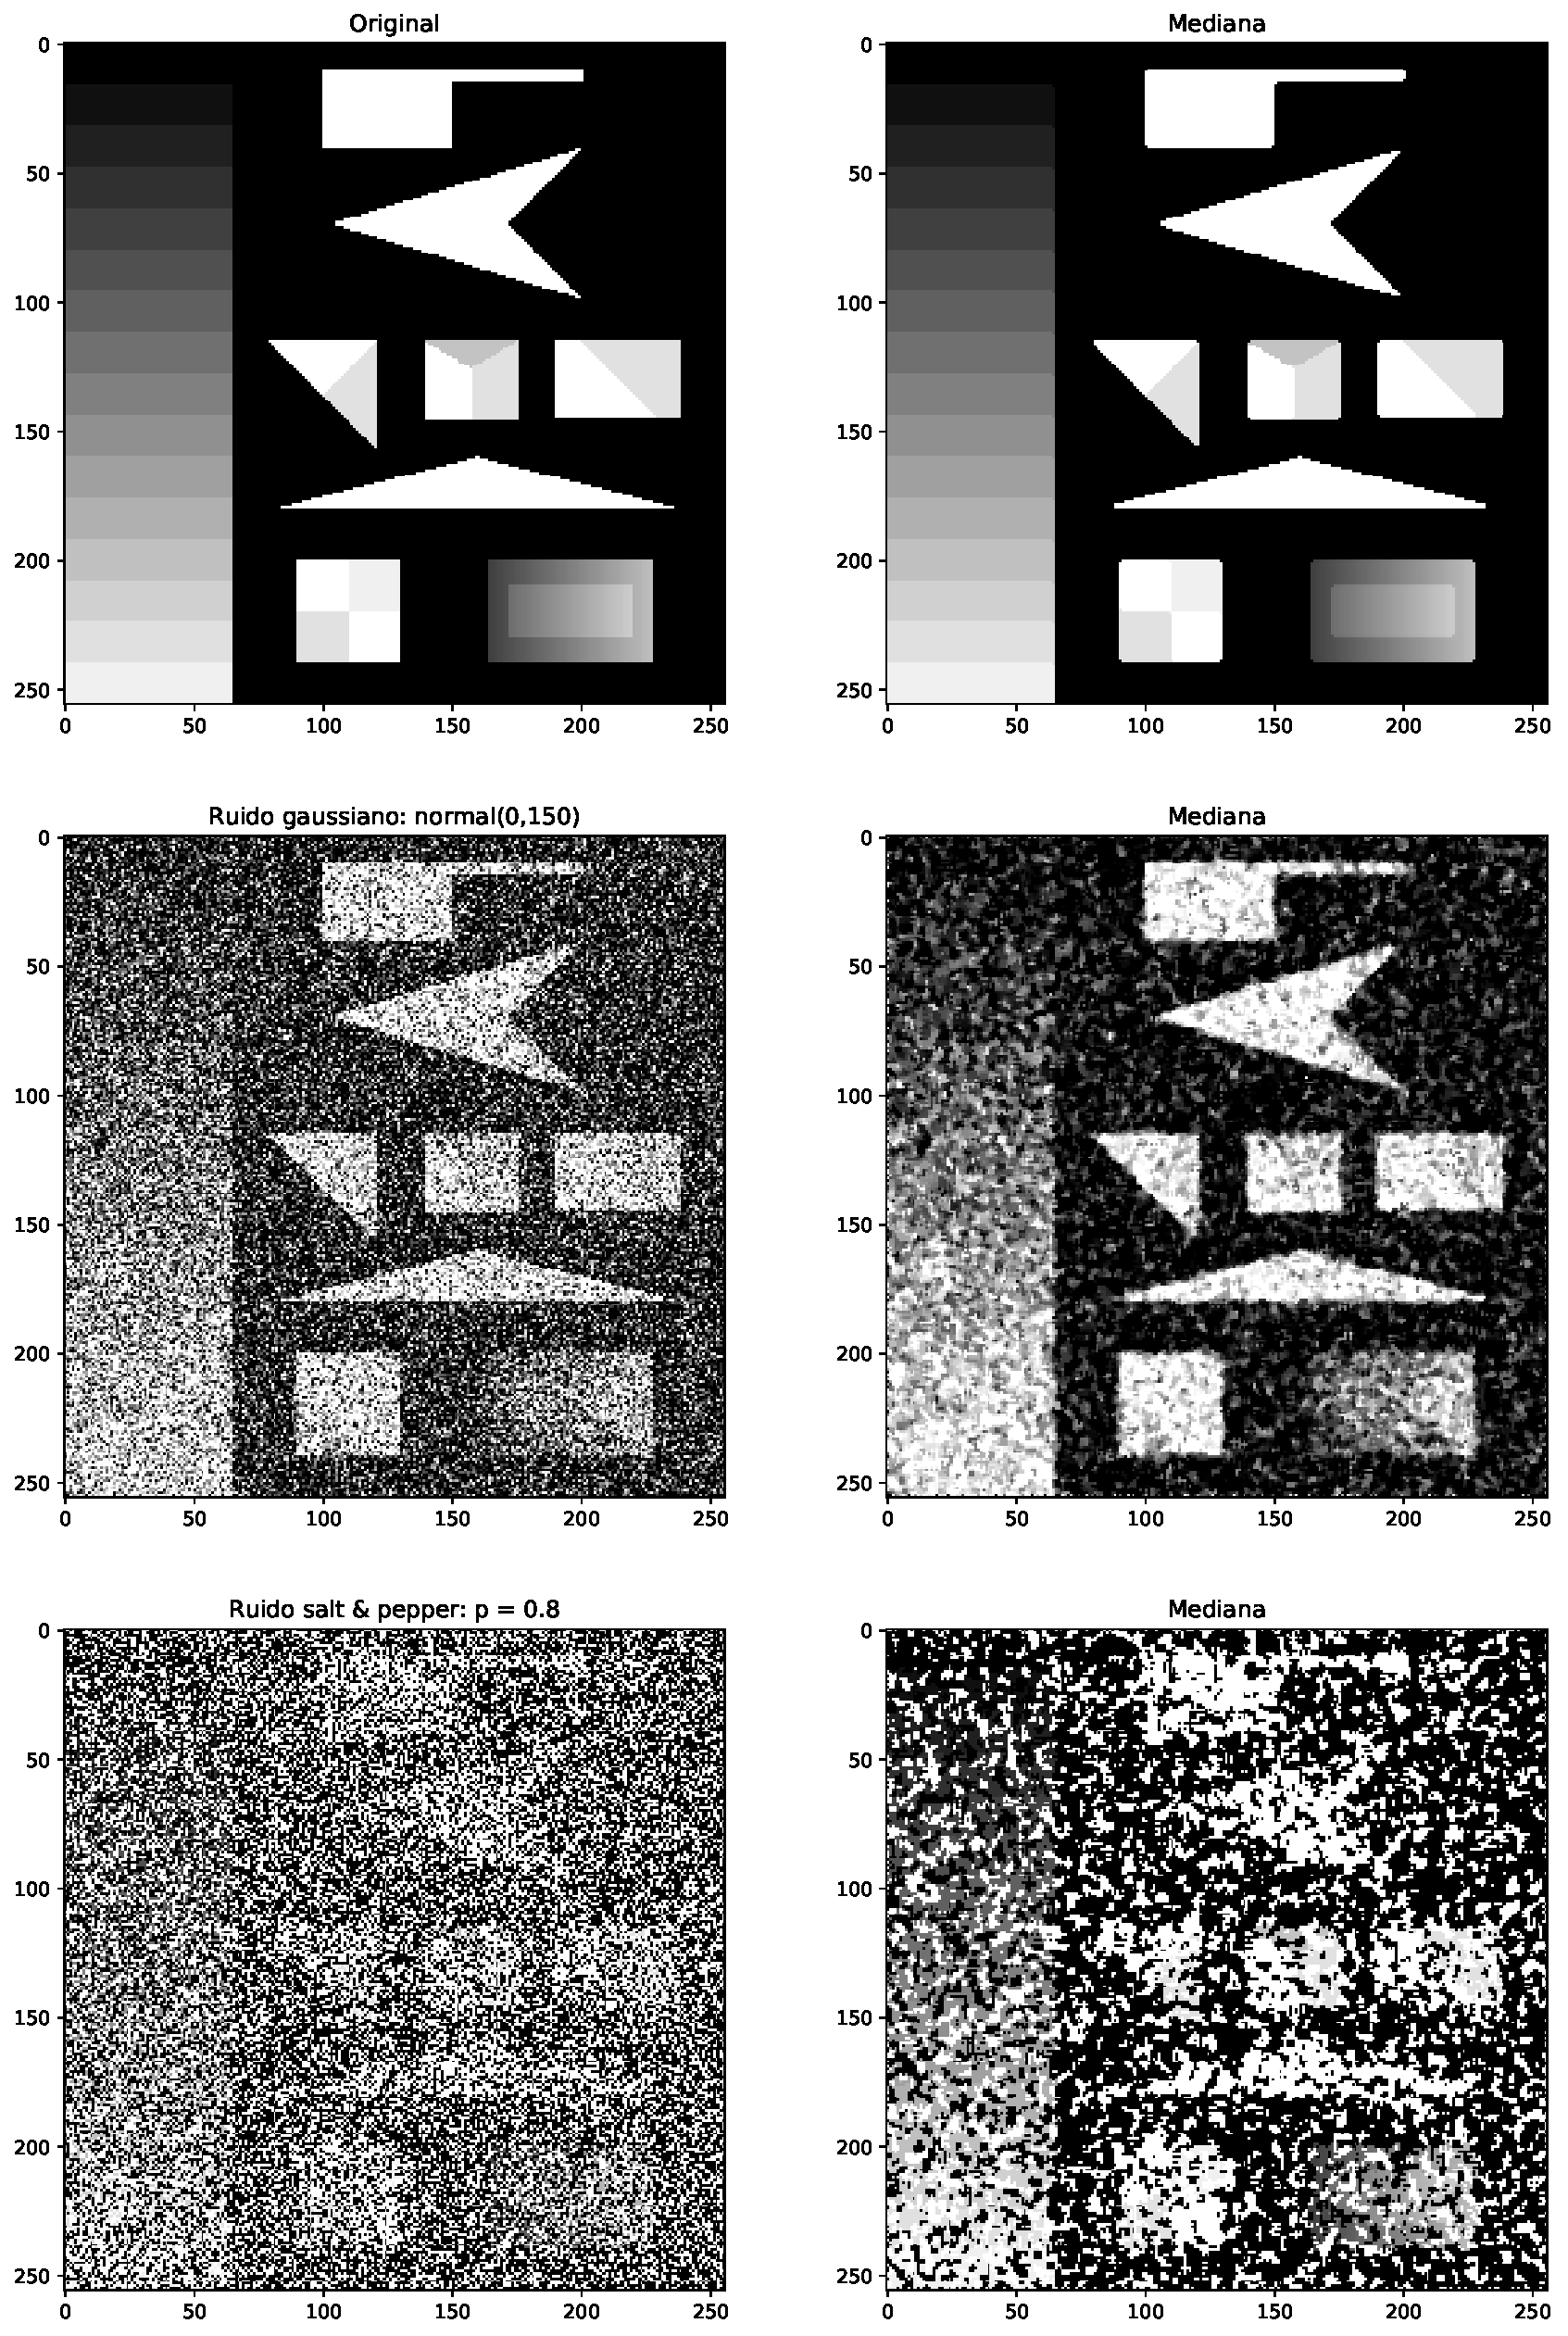
\includegraphics[height=10cm]{informe-imgs/ej6-3.jpg}
  \caption{\texttt{python3 practica5/ej5.py test.png 150 0.8}}
\end{figure}

\begin{figure}[H]
\centering
  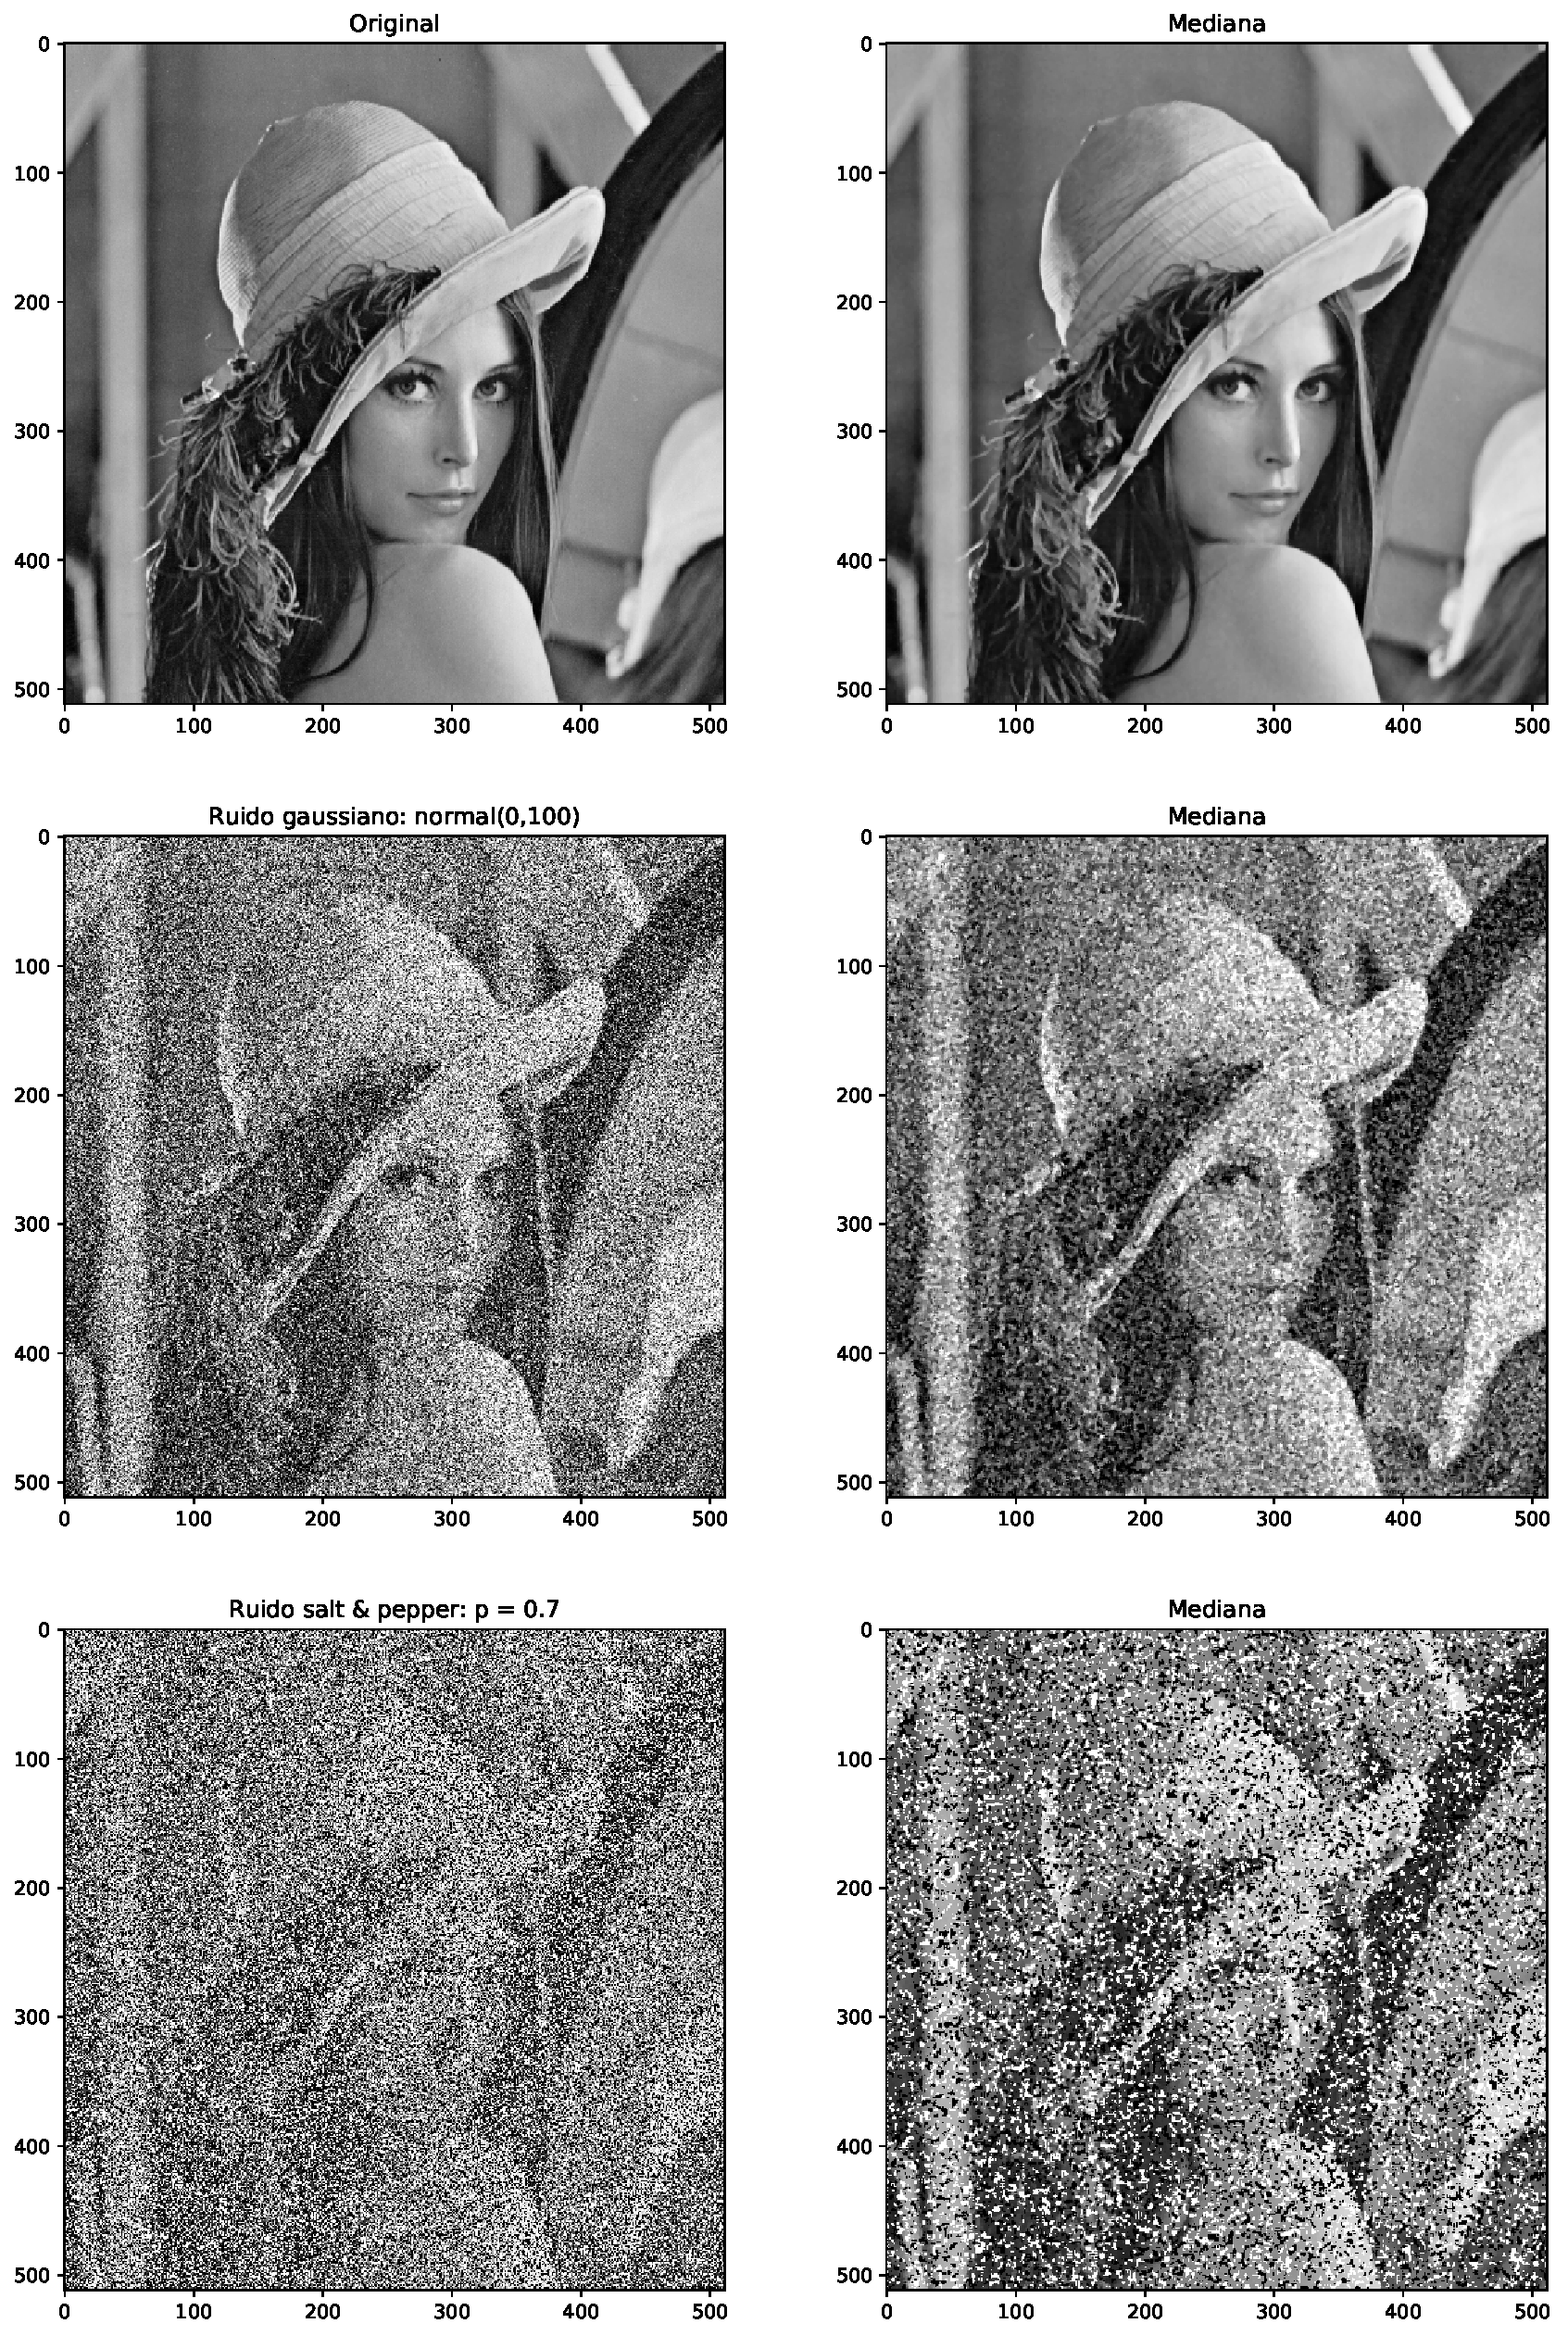
\includegraphics[height=10cm]{informe-imgs/ej6-4.jpg}
  \caption{\texttt{python3 practica5/ej5.py lena.png 100 0.7}}
\end{figure}

\newpage
\section{Ejercicios 7 y 8}

Filtros de detección de borde y su aplicación a imágenes con ruido.

Modo de uso
\begin{verbatim}
    python3 practica5/ej7.py <img> <roberts|prewitt|sobel> <param_gauss> <param_salt_pepper>
\end{verbatim}


\begin{figure}[H]
\centering
  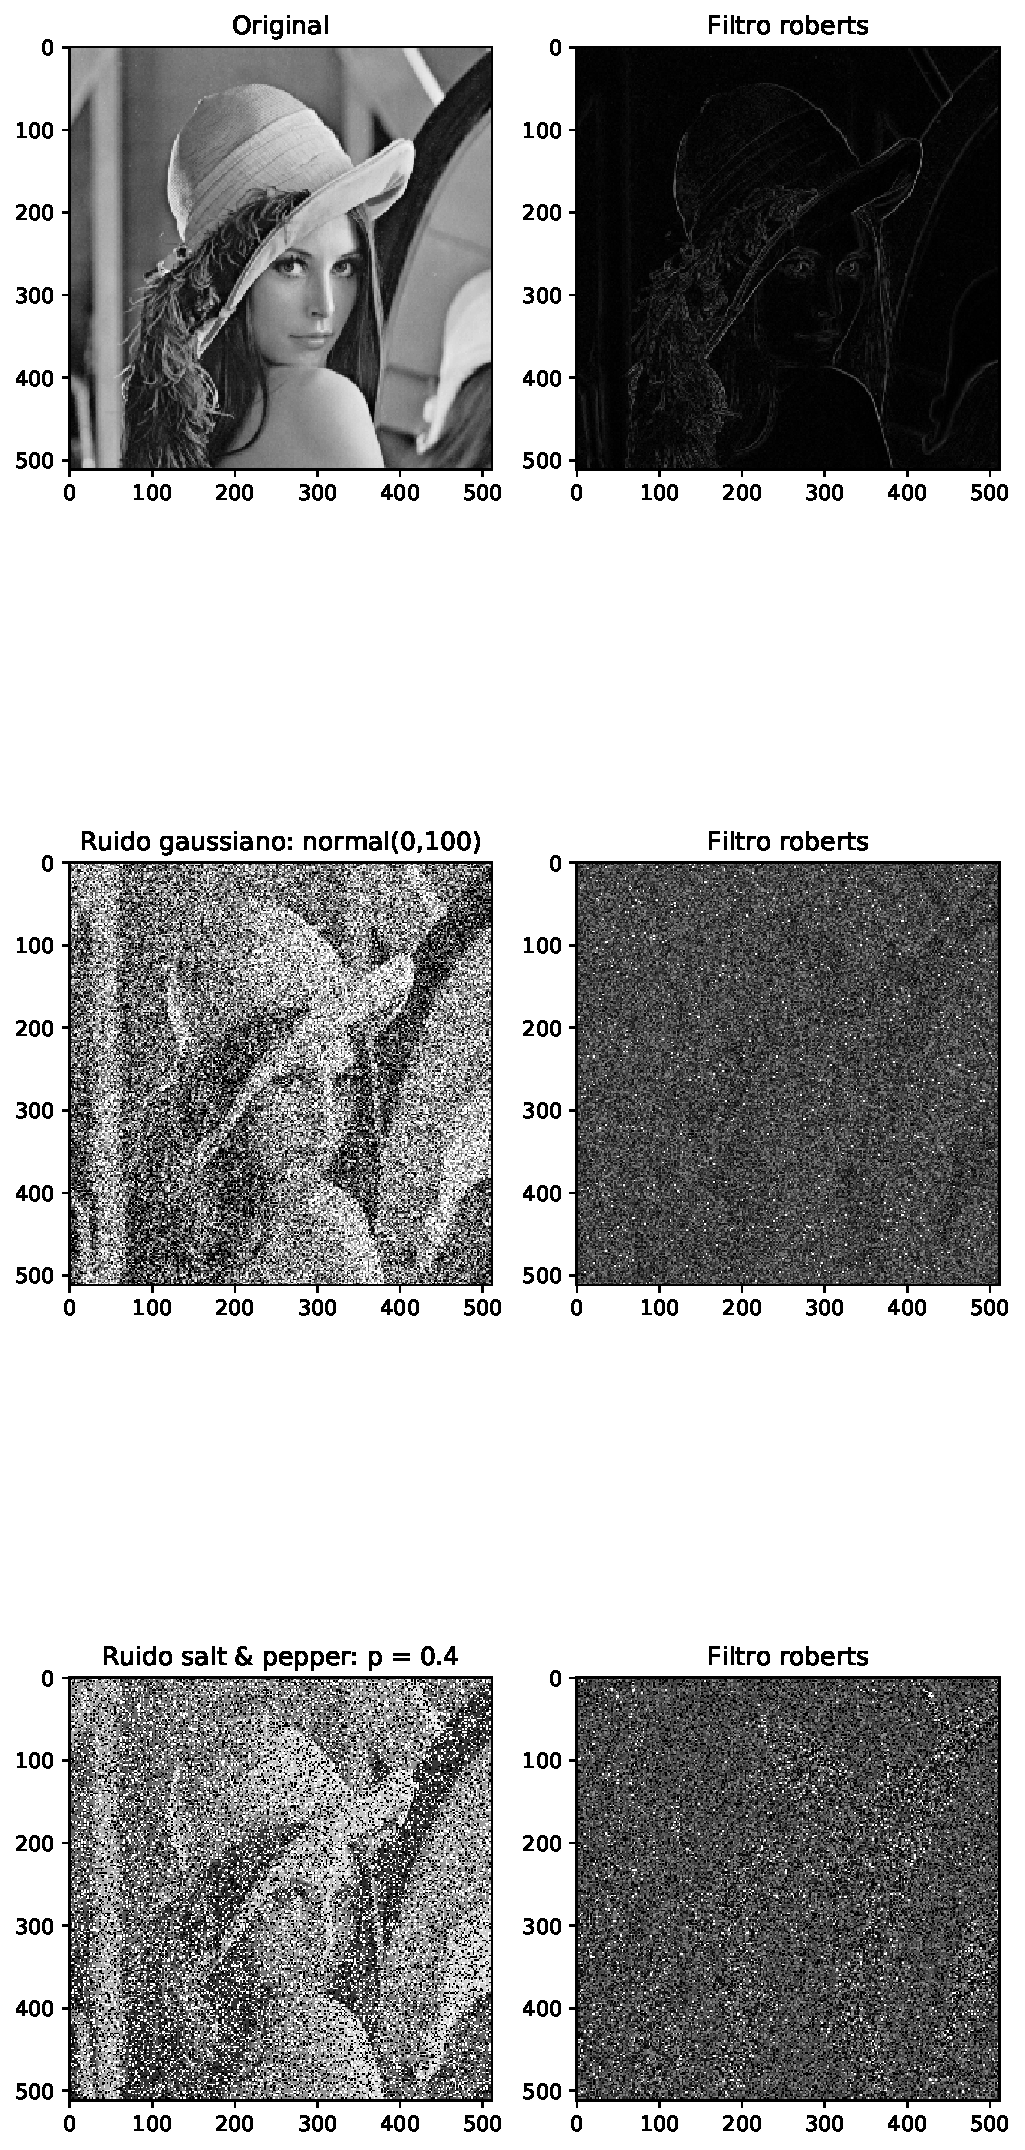
\includegraphics[height=10cm]{informe-imgs/ej7-3.jpg}
  \caption{\texttt{python3 practica5/ej7.py lena.png roberts 100 0.4}}
\end{figure}

\begin{figure}[H]
\centering
\begin{subfigure}{0.5\linewidth}
\centering
  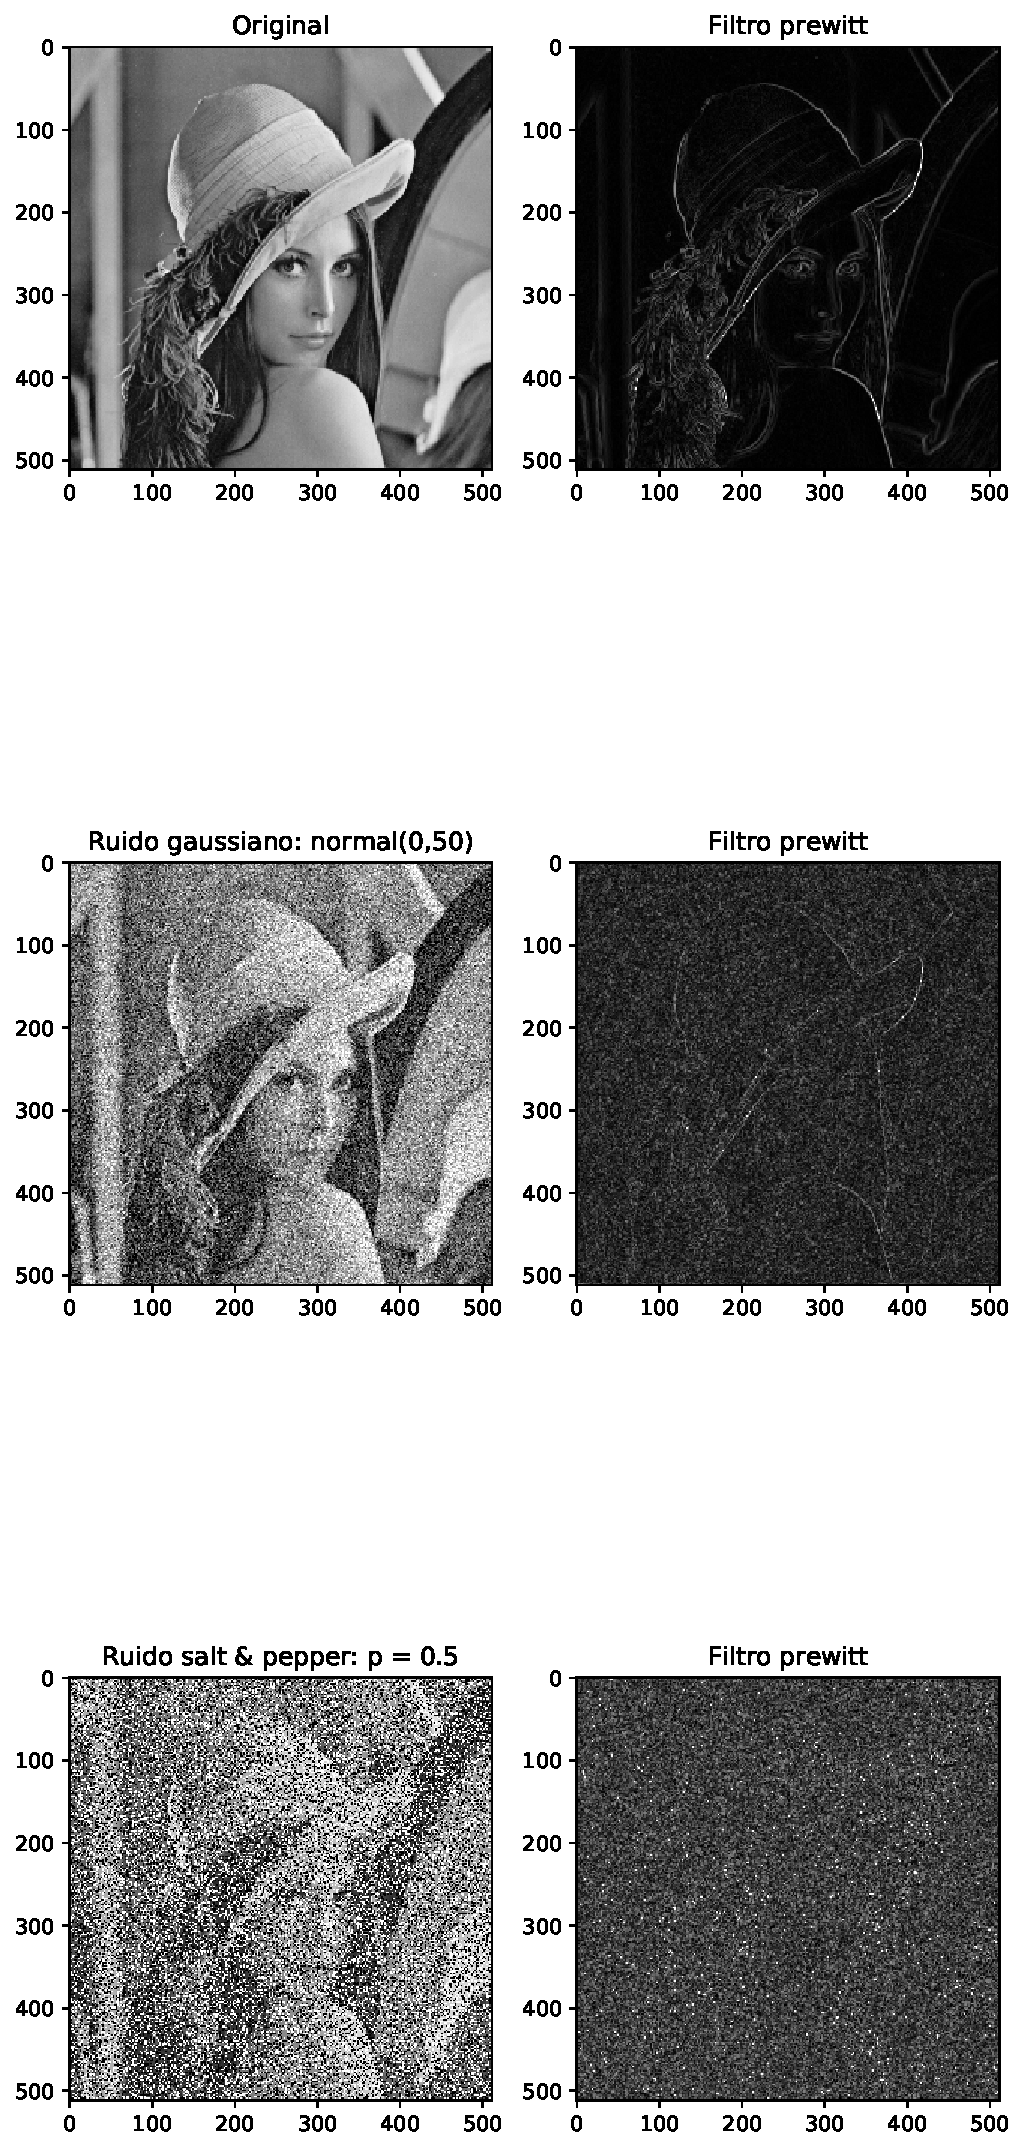
\includegraphics[height=10cm]{informe-imgs/ej7-2.jpg}
  \caption{\texttt{python3 practica5/ej7.py lena.png prewitt 50 0.5}}
\end{subfigure}%
\begin{subfigure}{0.5\linewidth}
\centering
  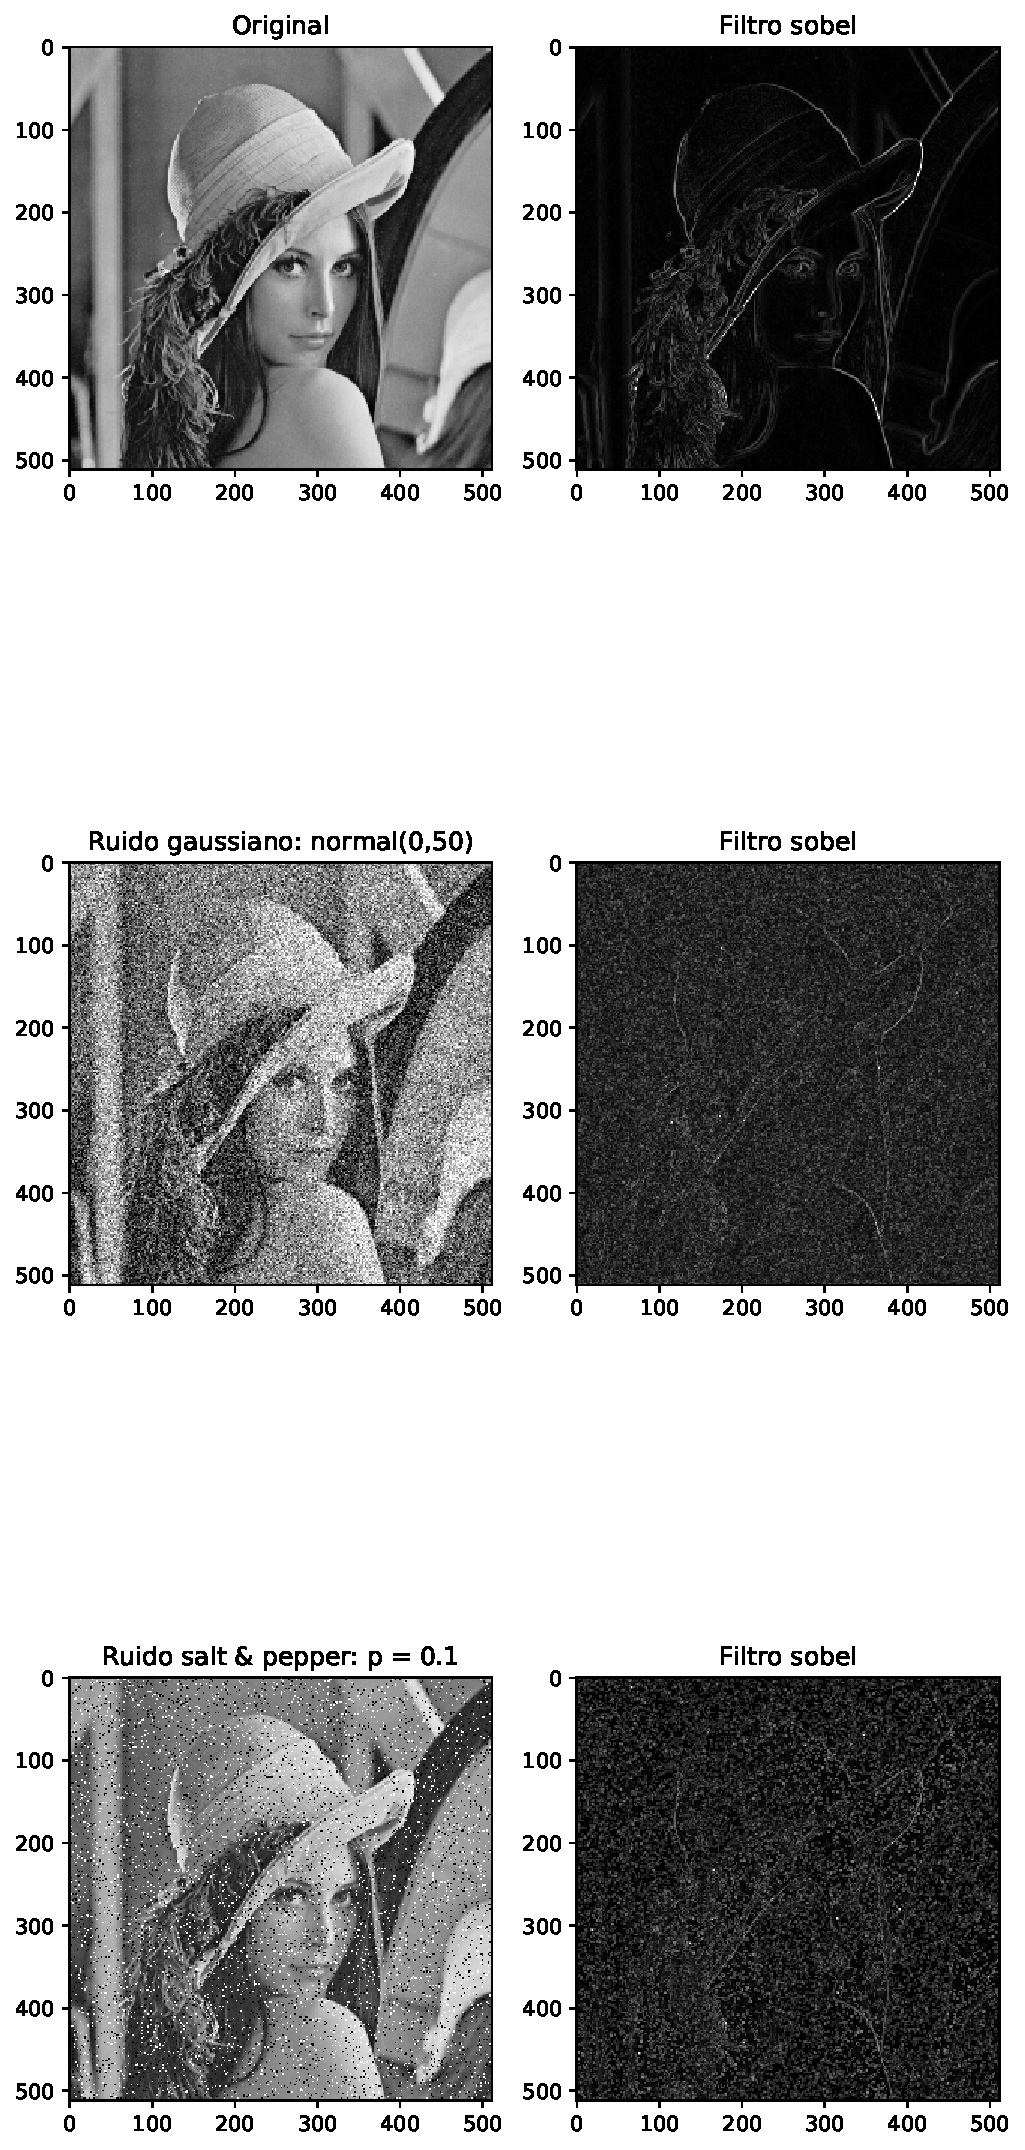
\includegraphics[height=10cm]{informe-imgs/ej7-1.jpg}
  \caption{\texttt{python3 practica5/ej7.py lena.png sobel 50 0.1}}
\end{subfigure}
\end{figure}


\begin{figure}[H]
\centering
  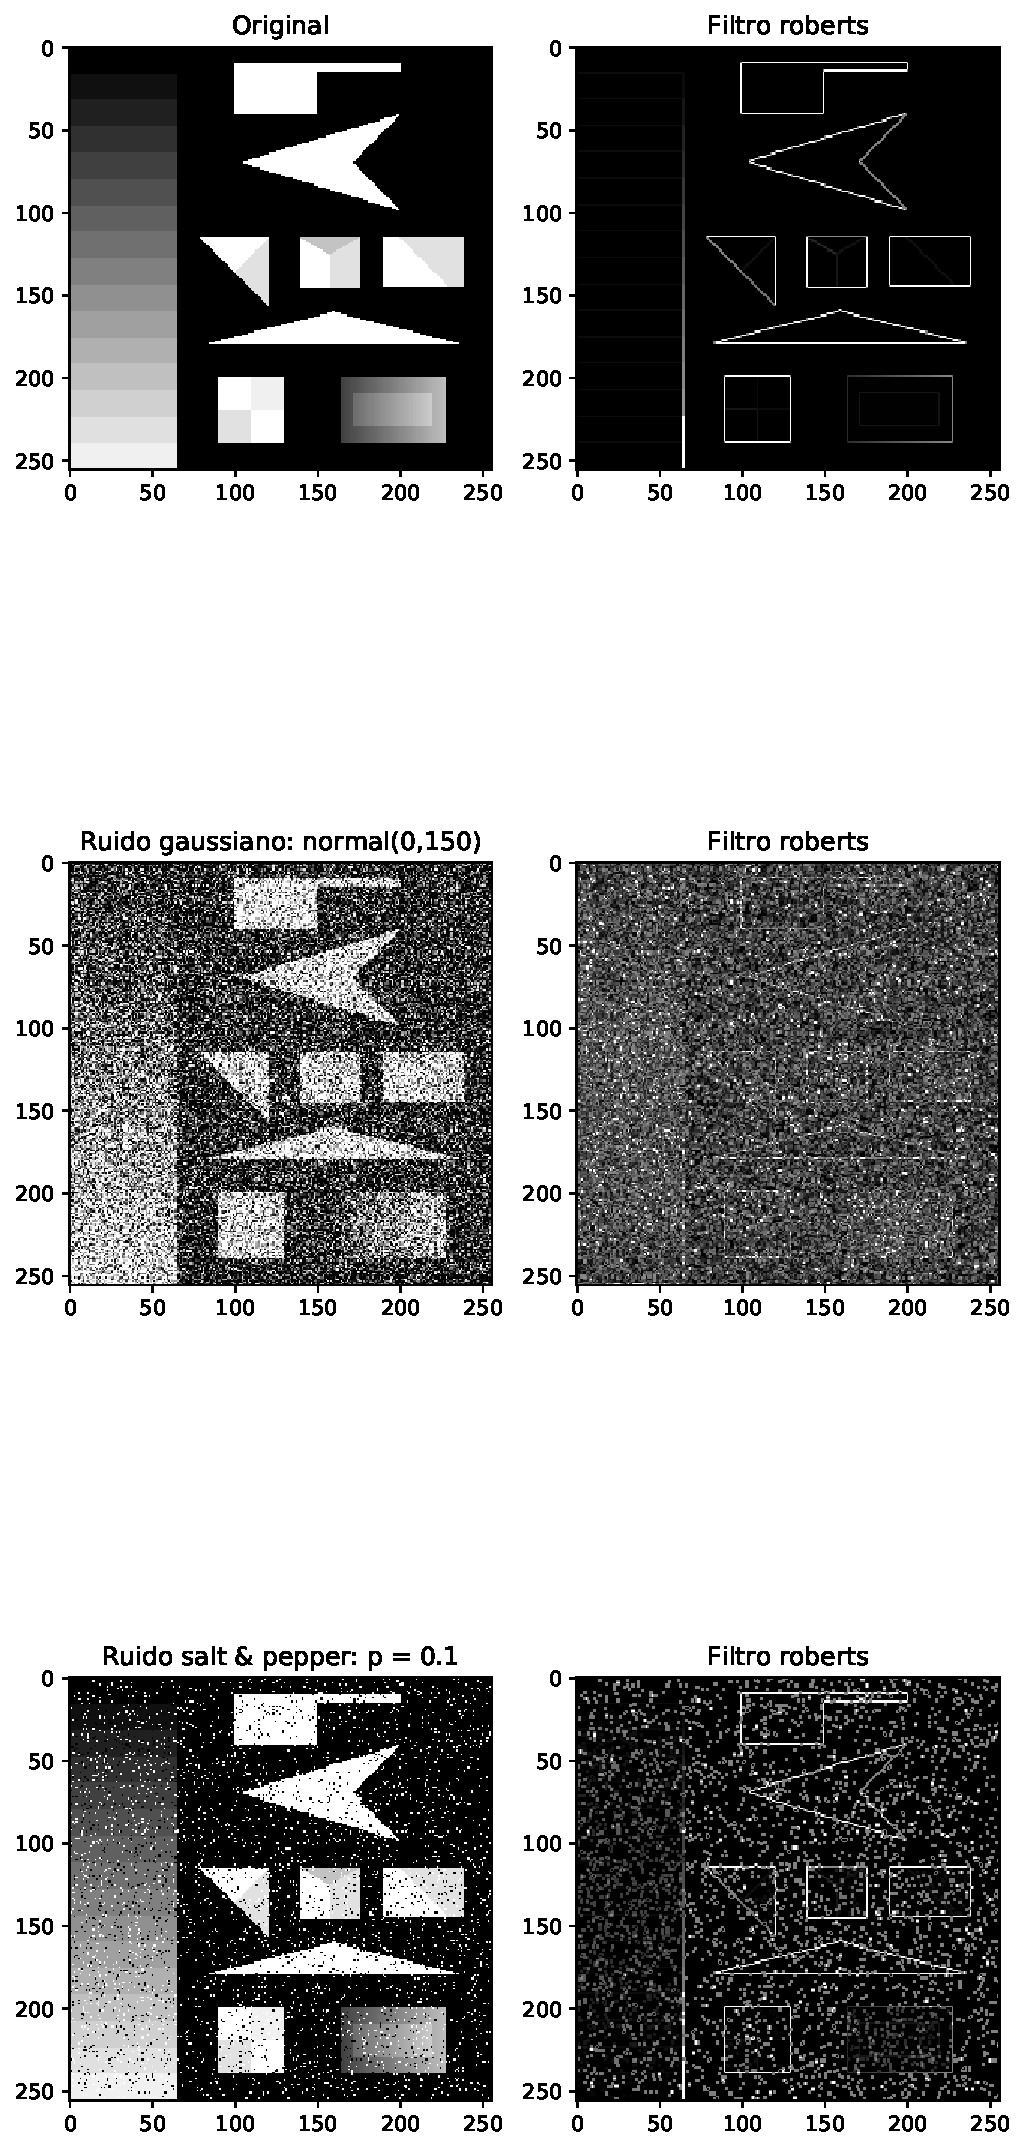
\includegraphics[height=10cm]{informe-imgs/ej7-4.jpg}
  \caption{\texttt{python3 practica5/ej7.py test.png roberts 150 0.1}}
\end{figure}

\begin{figure}[H]
\centering
\begin{subfigure}{0.5\linewidth}
\centering
  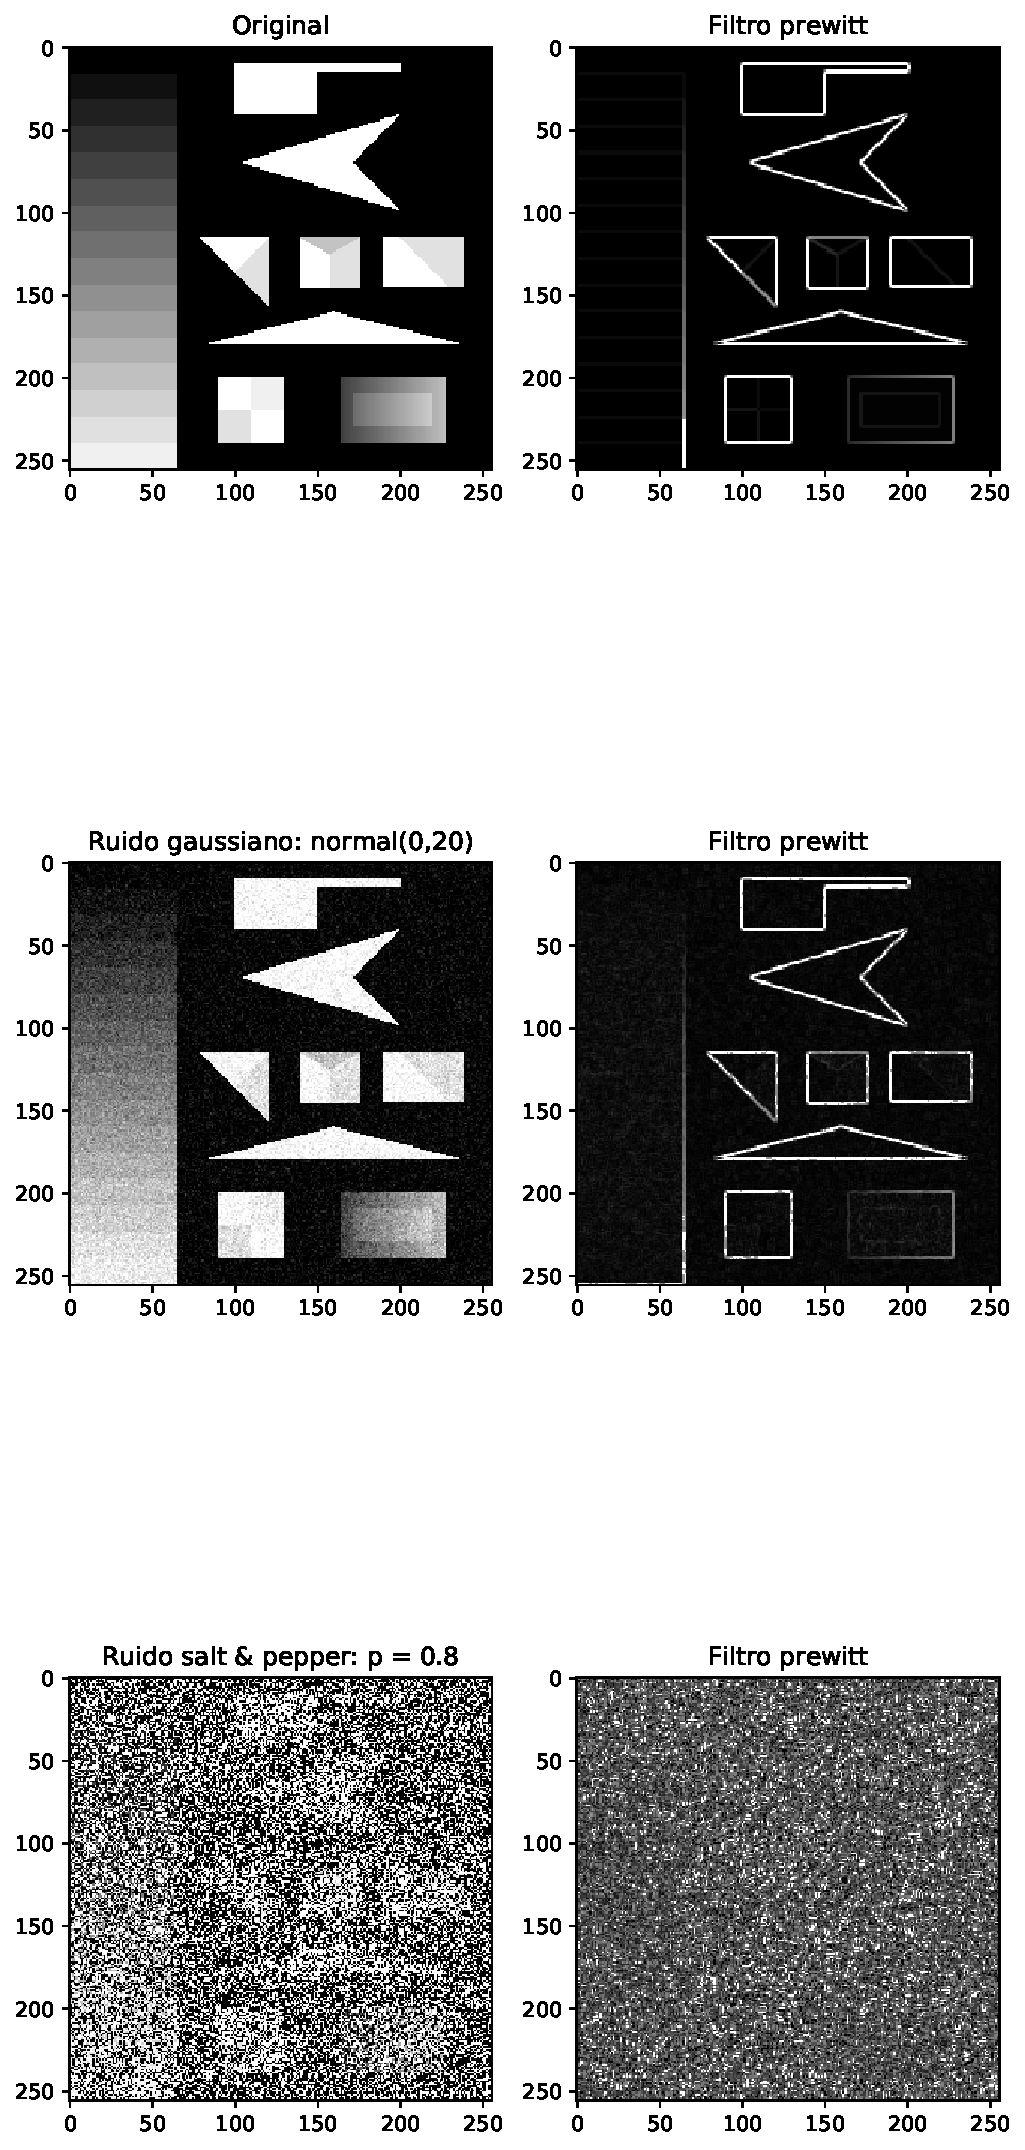
\includegraphics[height=10cm]{informe-imgs/ej7-5.jpg}
  \caption{\footnotesize{\texttt{python3 practica5/ej7.py test.png prewitt 20 0.8}}}
\end{subfigure}%
\begin{subfigure}{0.5\linewidth}
\centering
  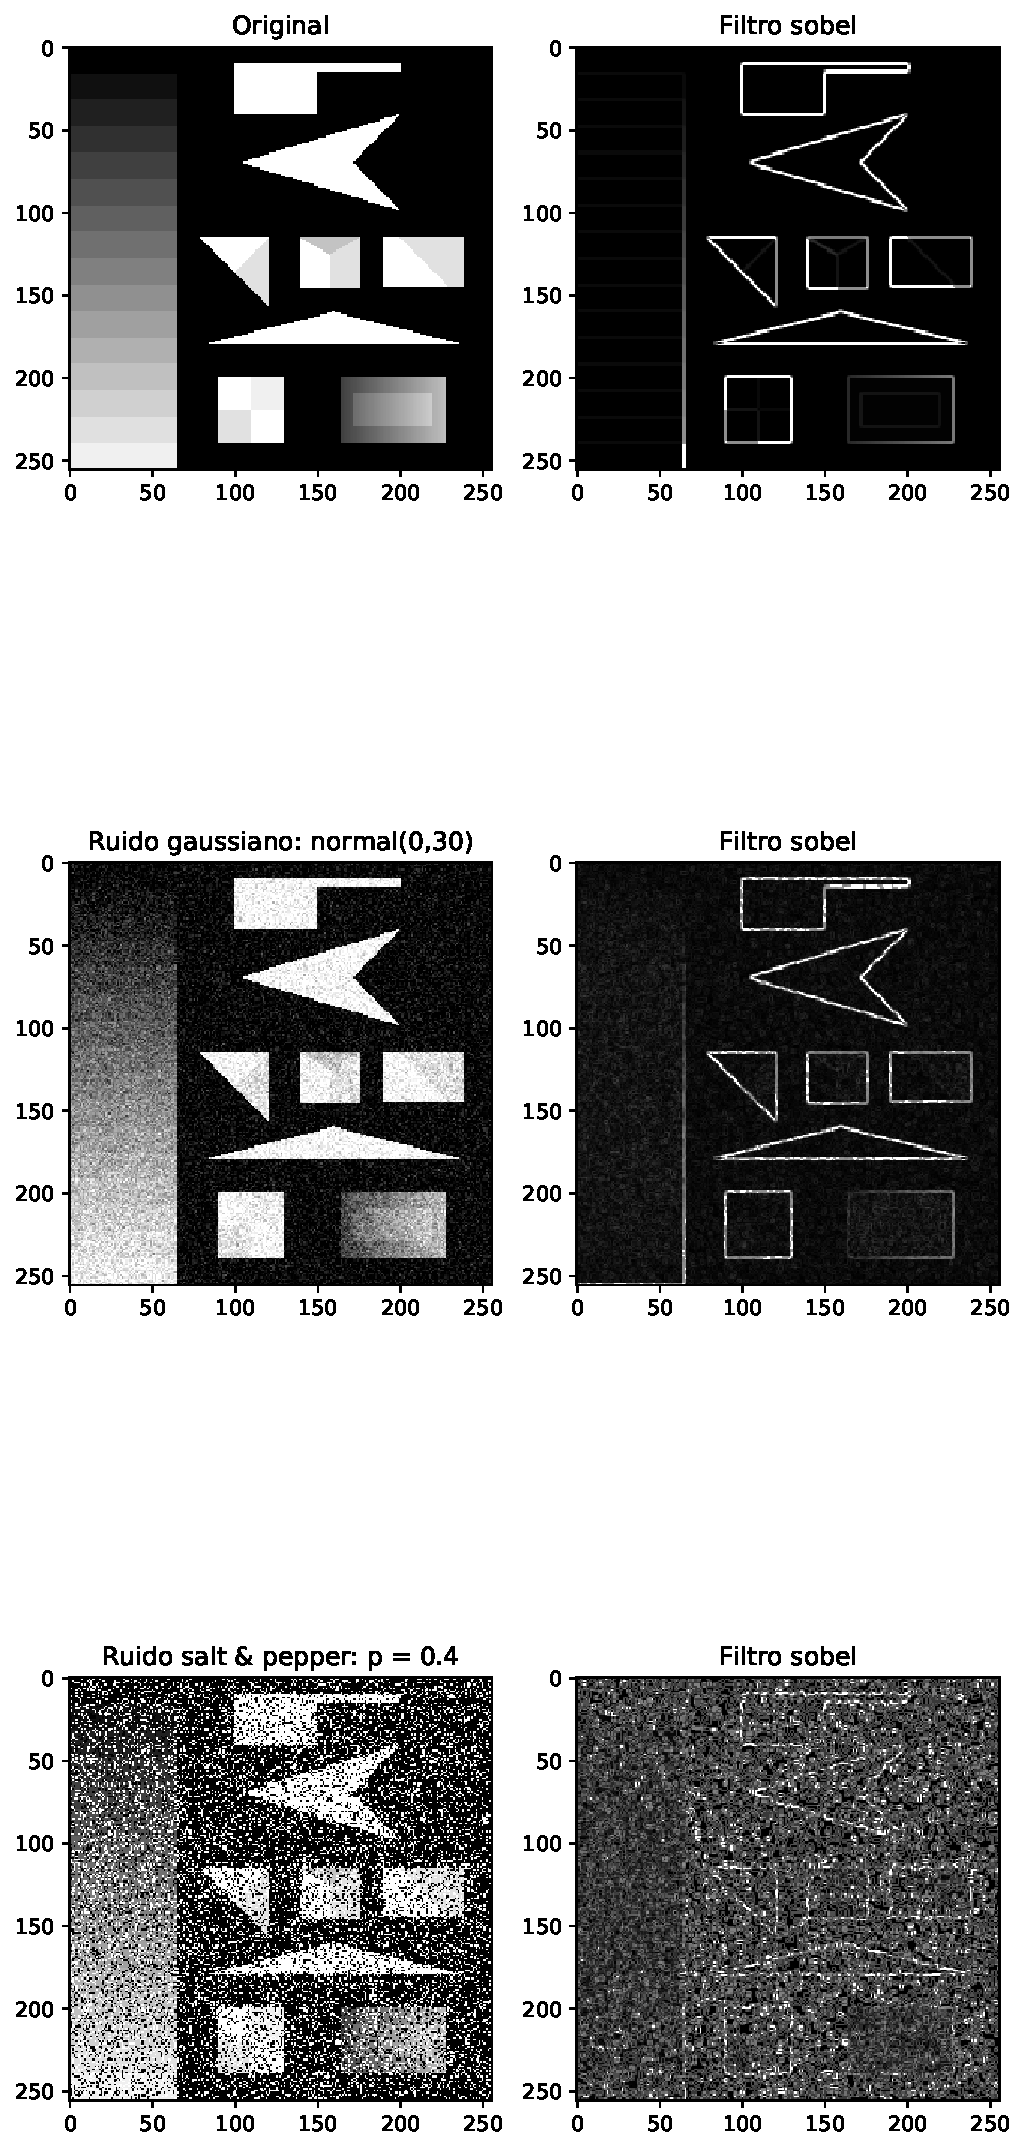
\includegraphics[height=10cm]{informe-imgs/ej7-6.jpg}
  \caption{\footnotesize{\texttt{python3 practica5/ej7.py test.png sobel 30 0.4}}}
\end{subfigure}
\end{figure}



\end{document}
